% Options for packages loaded elsewhere
\PassOptionsToPackage{unicode}{hyperref}
\PassOptionsToPackage{hyphens}{url}
\PassOptionsToPackage{dvipsnames,svgnames,x11names}{xcolor}
%
\documentclass[
  letterpaper,
]{report}

\usepackage{amsmath,amssymb}
\usepackage{lmodern}
\usepackage{iftex}
\ifPDFTeX
  \usepackage[T1]{fontenc}
  \usepackage[utf8]{inputenc}
  \usepackage{textcomp} % provide euro and other symbols
\else % if luatex or xetex
  \usepackage{unicode-math}
  \defaultfontfeatures{Scale=MatchLowercase}
  \defaultfontfeatures[\rmfamily]{Ligatures=TeX,Scale=1}
\fi
% Use upquote if available, for straight quotes in verbatim environments
\IfFileExists{upquote.sty}{\usepackage{upquote}}{}
\IfFileExists{microtype.sty}{% use microtype if available
  \usepackage[]{microtype}
  \UseMicrotypeSet[protrusion]{basicmath} % disable protrusion for tt fonts
}{}
\makeatletter
\@ifundefined{KOMAClassName}{% if non-KOMA class
  \IfFileExists{parskip.sty}{%
    \usepackage{parskip}
  }{% else
    \setlength{\parindent}{0pt}
    \setlength{\parskip}{6pt plus 2pt minus 1pt}}
}{% if KOMA class
  \KOMAoptions{parskip=half}}
\makeatother
\usepackage{xcolor}
\setlength{\emergencystretch}{3em} % prevent overfull lines
\setcounter{secnumdepth}{5}
% Make \paragraph and \subparagraph free-standing
\ifx\paragraph\undefined\else
  \let\oldparagraph\paragraph
  \renewcommand{\paragraph}[1]{\oldparagraph{#1}\mbox{}}
\fi
\ifx\subparagraph\undefined\else
  \let\oldsubparagraph\subparagraph
  \renewcommand{\subparagraph}[1]{\oldsubparagraph{#1}\mbox{}}
\fi

\usepackage{color}
\usepackage{fancyvrb}
\newcommand{\VerbBar}{|}
\newcommand{\VERB}{\Verb[commandchars=\\\{\}]}
\DefineVerbatimEnvironment{Highlighting}{Verbatim}{commandchars=\\\{\}}
% Add ',fontsize=\small' for more characters per line
\usepackage{framed}
\definecolor{shadecolor}{RGB}{241,243,245}
\newenvironment{Shaded}{\begin{snugshade}}{\end{snugshade}}
\newcommand{\AlertTok}[1]{\textcolor[rgb]{0.68,0.00,0.00}{#1}}
\newcommand{\AnnotationTok}[1]{\textcolor[rgb]{0.37,0.37,0.37}{#1}}
\newcommand{\AttributeTok}[1]{\textcolor[rgb]{0.40,0.45,0.13}{#1}}
\newcommand{\BaseNTok}[1]{\textcolor[rgb]{0.68,0.00,0.00}{#1}}
\newcommand{\BuiltInTok}[1]{\textcolor[rgb]{0.00,0.23,0.31}{#1}}
\newcommand{\CharTok}[1]{\textcolor[rgb]{0.13,0.47,0.30}{#1}}
\newcommand{\CommentTok}[1]{\textcolor[rgb]{0.37,0.37,0.37}{#1}}
\newcommand{\CommentVarTok}[1]{\textcolor[rgb]{0.37,0.37,0.37}{\textit{#1}}}
\newcommand{\ConstantTok}[1]{\textcolor[rgb]{0.56,0.35,0.01}{#1}}
\newcommand{\ControlFlowTok}[1]{\textcolor[rgb]{0.00,0.23,0.31}{#1}}
\newcommand{\DataTypeTok}[1]{\textcolor[rgb]{0.68,0.00,0.00}{#1}}
\newcommand{\DecValTok}[1]{\textcolor[rgb]{0.68,0.00,0.00}{#1}}
\newcommand{\DocumentationTok}[1]{\textcolor[rgb]{0.37,0.37,0.37}{\textit{#1}}}
\newcommand{\ErrorTok}[1]{\textcolor[rgb]{0.68,0.00,0.00}{#1}}
\newcommand{\ExtensionTok}[1]{\textcolor[rgb]{0.00,0.23,0.31}{#1}}
\newcommand{\FloatTok}[1]{\textcolor[rgb]{0.68,0.00,0.00}{#1}}
\newcommand{\FunctionTok}[1]{\textcolor[rgb]{0.28,0.35,0.67}{#1}}
\newcommand{\ImportTok}[1]{\textcolor[rgb]{0.00,0.46,0.62}{#1}}
\newcommand{\InformationTok}[1]{\textcolor[rgb]{0.37,0.37,0.37}{#1}}
\newcommand{\KeywordTok}[1]{\textcolor[rgb]{0.00,0.23,0.31}{#1}}
\newcommand{\NormalTok}[1]{\textcolor[rgb]{0.00,0.23,0.31}{#1}}
\newcommand{\OperatorTok}[1]{\textcolor[rgb]{0.37,0.37,0.37}{#1}}
\newcommand{\OtherTok}[1]{\textcolor[rgb]{0.00,0.23,0.31}{#1}}
\newcommand{\PreprocessorTok}[1]{\textcolor[rgb]{0.68,0.00,0.00}{#1}}
\newcommand{\RegionMarkerTok}[1]{\textcolor[rgb]{0.00,0.23,0.31}{#1}}
\newcommand{\SpecialCharTok}[1]{\textcolor[rgb]{0.37,0.37,0.37}{#1}}
\newcommand{\SpecialStringTok}[1]{\textcolor[rgb]{0.13,0.47,0.30}{#1}}
\newcommand{\StringTok}[1]{\textcolor[rgb]{0.13,0.47,0.30}{#1}}
\newcommand{\VariableTok}[1]{\textcolor[rgb]{0.07,0.07,0.07}{#1}}
\newcommand{\VerbatimStringTok}[1]{\textcolor[rgb]{0.13,0.47,0.30}{#1}}
\newcommand{\WarningTok}[1]{\textcolor[rgb]{0.37,0.37,0.37}{\textit{#1}}}

\providecommand{\tightlist}{%
  \setlength{\itemsep}{0pt}\setlength{\parskip}{0pt}}\usepackage{longtable,booktabs,array}
\usepackage{calc} % for calculating minipage widths
% Correct order of tables after \paragraph or \subparagraph
\usepackage{etoolbox}
\makeatletter
\patchcmd\longtable{\par}{\if@noskipsec\mbox{}\fi\par}{}{}
\makeatother
% Allow footnotes in longtable head/foot
\IfFileExists{footnotehyper.sty}{\usepackage{footnotehyper}}{\usepackage{footnote}}
\makesavenoteenv{longtable}
\usepackage{graphicx}
\makeatletter
\def\maxwidth{\ifdim\Gin@nat@width>\linewidth\linewidth\else\Gin@nat@width\fi}
\def\maxheight{\ifdim\Gin@nat@height>\textheight\textheight\else\Gin@nat@height\fi}
\makeatother
% Scale images if necessary, so that they will not overflow the page
% margins by default, and it is still possible to overwrite the defaults
% using explicit options in \includegraphics[width, height, ...]{}
\setkeys{Gin}{width=\maxwidth,height=\maxheight,keepaspectratio}
% Set default figure placement to htbp
\makeatletter
\def\fps@figure{htbp}
\makeatother
\newlength{\cslhangindent}
\setlength{\cslhangindent}{1.5em}
\newlength{\csllabelwidth}
\setlength{\csllabelwidth}{3em}
\newlength{\cslentryspacingunit} % times entry-spacing
\setlength{\cslentryspacingunit}{\parskip}
\newenvironment{CSLReferences}[2] % #1 hanging-ident, #2 entry spacing
 {% don't indent paragraphs
  \setlength{\parindent}{0pt}
  % turn on hanging indent if param 1 is 1
  \ifodd #1
  \let\oldpar\par
  \def\par{\hangindent=\cslhangindent\oldpar}
  \fi
  % set entry spacing
  \setlength{\parskip}{#2\cslentryspacingunit}
 }%
 {}
\usepackage{calc}
\newcommand{\CSLBlock}[1]{#1\hfill\break}
\newcommand{\CSLLeftMargin}[1]{\parbox[t]{\csllabelwidth}{#1}}
\newcommand{\CSLRightInline}[1]{\parbox[t]{\linewidth - \csllabelwidth}{#1}\break}
\newcommand{\CSLIndent}[1]{\hspace{\cslhangindent}#1}

\usepackage{booktabs}
\usepackage{longtable}
\usepackage{array}
\usepackage{multirow}
\usepackage{wrapfig}
\usepackage{float}
\usepackage{colortbl}
\usepackage{pdflscape}
\usepackage{tabu}
\usepackage{threeparttable}
\usepackage{threeparttablex}
\usepackage[normalem]{ulem}
\usepackage{makecell}
\usepackage{xcolor}
\makeatletter
\makeatother
\makeatletter
\@ifpackageloaded{bookmark}{}{\usepackage{bookmark}}
\makeatother
\makeatletter
\@ifpackageloaded{caption}{}{\usepackage{caption}}
\AtBeginDocument{%
\ifdefined\contentsname
  \renewcommand*\contentsname{Table of contents}
\else
  \newcommand\contentsname{Table of contents}
\fi
\ifdefined\listfigurename
  \renewcommand*\listfigurename{List of Figures}
\else
  \newcommand\listfigurename{List of Figures}
\fi
\ifdefined\listtablename
  \renewcommand*\listtablename{List of Tables}
\else
  \newcommand\listtablename{List of Tables}
\fi
\ifdefined\figurename
  \renewcommand*\figurename{Figure}
\else
  \newcommand\figurename{Figure}
\fi
\ifdefined\tablename
  \renewcommand*\tablename{Table}
\else
  \newcommand\tablename{Table}
\fi
}
\@ifpackageloaded{float}{}{\usepackage{float}}
\floatstyle{ruled}
\@ifundefined{c@chapter}{\newfloat{codelisting}{h}{lop}}{\newfloat{codelisting}{h}{lop}[chapter]}
\floatname{codelisting}{Listing}
\newcommand*\listoflistings{\listof{codelisting}{List of Listings}}
\makeatother
\makeatletter
\@ifpackageloaded{caption}{}{\usepackage{caption}}
\@ifpackageloaded{subcaption}{}{\usepackage{subcaption}}
\makeatother
\makeatletter
\@ifpackageloaded{tcolorbox}{}{\usepackage[many]{tcolorbox}}
\makeatother
\makeatletter
\@ifundefined{shadecolor}{\definecolor{shadecolor}{rgb}{.97, .97, .97}}
\makeatother
\makeatletter
\makeatother
\ifLuaTeX
  \usepackage{selnolig}  % disable illegal ligatures
\fi
\IfFileExists{bookmark.sty}{\usepackage{bookmark}}{\usepackage{hyperref}}
\IfFileExists{xurl.sty}{\usepackage{xurl}}{} % add URL line breaks if available
\urlstyle{same} % disable monospaced font for URLs
\hypersetup{
  pdftitle={Defining Data Science},
  pdfauthor={Xinrui WANG and Tsai-Chun TSOU},
  colorlinks=true,
  linkcolor={blue},
  filecolor={Maroon},
  citecolor={Blue},
  urlcolor={Blue},
  pdfcreator={LaTeX via pandoc}}

\title{Defining Data Science}
\usepackage{etoolbox}
\makeatletter
\providecommand{\subtitle}[1]{% add subtitle to \maketitle
  \apptocmd{\@title}{\par {\large #1 \par}}{}{}
}
\makeatother
\subtitle{A Case Study in Australia}
\author{Xinrui WANG and Tsai-Chun TSOU}
\date{28 October 2022}

\begin{document}
\maketitle
\ifdefined\Shaded\renewenvironment{Shaded}{\begin{tcolorbox}[sharp corners, boxrule=0pt, interior hidden, frame hidden, borderline west={3pt}{0pt}{shadecolor}, breakable, enhanced]}{\end{tcolorbox}}\fi

\renewcommand*\contentsname{Table of contents}
{
\hypersetup{linkcolor=}
\setcounter{tocdepth}{2}
\tableofcontents
}
\bookmarksetup{startatroot}

\hypertarget{abstract}{%
\chapter*{Abstract}\label{abstract}}
\addcontentsline{toc}{chapter}{Abstract}

Universities are increasingly offering degrees that specialise in the
so-called ``Data Science'' but what is Data Science and what skill are
students expected to master in these degrees? The Australian
Mathematical Sciences Institute (AMSI) and the Statistical Society of
Australia (SSA) are conducting a review of role of of Data Science in
Australia universities using
\href{https://amsi.org.au/amsi-ssa-data-science-review/}{surveys} and
focus groups. Our research attempts to tackle this topic by using data
available from public resources. More specifically, we collected unit
description and learning objectives/outcomes in Master of Data Science
in the Group of Eight (Go8) Universities and job description of data
scientist roles from seek.com.au available on from
\href{https://www.kaggle.com/code/nomilk/exploring-2-years-of-data-scientist-job-listings/data}{Kaggle}.
We used the data to decompose the core disciplines involved in the
degree as well the type of skill sets that may be required. To expand on
the initial exploratory data analysis, we also build Latent Dirichlet
Allocation models to construct our own text corpus.

From the exploratory data analysis, we observe a lack of homogeneity of
the composition of unit structure across the Go8 universities. The
inconsistent data metrics made it difficult to draw direct comparison
between the employer data and university data. Nonetheless we were able
to conclude that computational components are more prominent in data
science for both the university and employer perspectives.

\bookmarksetup{startatroot}

\hypertarget{introduction}{%
\chapter{Introduction}\label{introduction}}

Data Science has ranked as one of the most in-demand jobs in Australia
in recent consecutive years. As demands steadily grows, students are
also increasingly interested in Data Science degrees, yet recruiters
still seem to struggle to fill up data science positions. This leads to
our main question: what is Data Science? Is there a shared structure or
skill set of Data Science courses offered at Australian universities?
Are students and employers' perception of data science similar? To
answer these questions, we looked at data from both University and
Employer perspectives.

There is no readily available data from Australian universities, so we
had to collect our own data set through web scraping. The initial target
was to collect data from all universities in Australia including both
undergraduate and postgraduate courses, however, due to time constrain,
the data collected for this project only contains Master of Data Science
courses from the Group of Eight (Go8) universities. The data on job
description (which we refer to as ``employer data'') was retrieved from
\href{(https://www.kaggle.com/code/nomilk/exploring-2-years-of-data-scientist-job-listings/data)}{Data
Scientist Job Listings} on Kaggle.

By exploring the current situation and potentially a definition of Data
Science in Australia from both the university and employer perspectives,
the findings would help students and recruiters have a clearer picture
of what to expect, as well as raising attentions and awareness to
potential gaps between employer demands and university offerings.

The project was conducted in three main phases. The first phase is data
collection (Chapter 2 \& Chapter 3). Phase two is exploratory data
analysis on the university data (Chapter 5) and on employer data
(Chapter 6). Details of some pre-processing procedures are included in
Chapter 4. Phase three is topic modelling (Chapter 7 \& Chapter 8) where
we built our own text corpus and group words from the data sets in
attempt to find more meaningful results.

Our concluding summary and thoughts on the future direction of this
project is in Chapter 9.

\part{Data Collection}

\hypertarget{sec-unidata}{%
\chapter{University Data}\label{sec-unidata}}

\hypertarget{web-scraping}{%
\section{Web Scraping}\label{web-scraping}}

In order to explore the Data Science degrees in Australian Universities,
we compiled a list of universities in Australia and the Data Science or
related degrees they offered, then web scraped required information from
each university's website using the R programming language (R Core Team
2021). In total, we collected 298 units from eight postgraduate courses
in Data Science across all Group of Eight (Go8) universities.

To start off the project, Dr.~Tanaka provided sample code for data
scraping using Monash Handbook as an example. Libraries \texttt{rvest}
and \texttt{RSelenium} are two of the main tools. Initially, we studied
her code and then tried to replicate her code to be applied to other
university's websites.

The flow of the data scraping is as follow (example code from
\texttt{uom-master-datasci.qmd}):

\begin{enumerate}
\def\labelenumi{\arabic{enumi}.}
\tightlist
\item
  Identify the main page (url) where the degree information is
  contained, which usually is the most updated version of the handbook.
\end{enumerate}

\begin{Shaded}
\begin{Highlighting}[]
\NormalTok{remDr}\SpecialCharTok{$}\FunctionTok{navigate}\NormalTok{(}\StringTok{"https://handbook.unimelb.edu.au/2022/courses/mc{-}datasc/course{-}structure"}\NormalTok{)}
\NormalTok{sub\_list }\OtherTok{\textless{}{-}} \FunctionTok{read\_html}\NormalTok{(remDr}\SpecialCharTok{$}\FunctionTok{getPageSource}\NormalTok{()[[}\DecValTok{1}\NormalTok{]])}
\end{Highlighting}
\end{Shaded}

\begin{enumerate}
\def\labelenumi{\arabic{enumi}.}
\setcounter{enumi}{1}
\tightlist
\item
  Use functions from \texttt{rvest} to retrieve all the course unit code
  (or course unit url). Retrieve the degree code and formal degree name
  and save it for later.
\end{enumerate}

\begin{Shaded}
\begin{Highlighting}[]
\NormalTok{curriculum }\OtherTok{\textless{}{-}}\NormalTok{ sub\_list }\SpecialCharTok{\%\textgreater{}\%} 
      \FunctionTok{html\_element}\NormalTok{(}\StringTok{"\#top"}\NormalTok{) }\SpecialCharTok{\%\textgreater{}\%} 
      \FunctionTok{html\_element}\NormalTok{(}\StringTok{".mobile{-}wrap"}\NormalTok{) }\SpecialCharTok{\%\textgreater{}\%} 
      \FunctionTok{html\_elements}\NormalTok{(}\StringTok{"table"}\NormalTok{) }\SpecialCharTok{\%\textgreater{}\%} 
      \FunctionTok{html\_elements}\NormalTok{(}\StringTok{"a"}\NormalTok{) }\SpecialCharTok{\%\textgreater{}\%} 
      \FunctionTok{html\_attr}\NormalTok{(}\StringTok{"href"}\NormalTok{)}
\end{Highlighting}
\end{Shaded}

\begin{enumerate}
\def\labelenumi{\arabic{enumi}.}
\setcounter{enumi}{2}
\item
  Use \texttt{RSelenium} functions and course unit information, to
  direct R to the unit information page.
\item
  Retrieve the following information from the page using rvest
  functions:

  \begin{itemize}
  \tightlist
  \item
    Unit Name
  \item
    Unit Code
  \item
    Unit Overview
  \item
    Unit Learning Outcome
  \item
    Unit Prohibition/ Pre-requisite/ Co-requisite
  \end{itemize}
\item
  Repeat step 3 \& 4 with loop function.
\end{enumerate}

\begin{Shaded}
\begin{Highlighting}[]
\ControlFlowTok{for}\NormalTok{(unit }\ControlFlowTok{in}\NormalTok{ curriculum) \{}
\NormalTok{      remDr}\SpecialCharTok{$}\FunctionTok{navigate}\NormalTok{(}\FunctionTok{glue}\NormalTok{(}\StringTok{"\{baseurl\}\{unit\}"}\NormalTok{))}
      \FunctionTok{wait\_time}\NormalTok{()}
\NormalTok{      unit\_html }\OtherTok{\textless{}{-}} \FunctionTok{read\_html}\NormalTok{(remDr}\SpecialCharTok{$}\FunctionTok{getPageSource}\NormalTok{()[[}\DecValTok{1}\NormalTok{]])}
      
      \CommentTok{\# unit name}
\NormalTok{      subject\_text }\OtherTok{\textless{}{-}}\NormalTok{ unit\_html }\SpecialCharTok{\%\textgreater{}\%} 
        \FunctionTok{html\_element}\NormalTok{(}\StringTok{"h1"}\NormalTok{) }\SpecialCharTok{\%\textgreater{}\%} 
        \FunctionTok{html\_text}\NormalTok{()}
\NormalTok{        ...}
\end{Highlighting}
\end{Shaded}

\begin{enumerate}
\def\labelenumi{\arabic{enumi}.}
\setcounter{enumi}{5}
\tightlist
\item
  Compile all the retrieved data from the University into a single data
  table and export it as a csv file.
\end{enumerate}

\begin{Shaded}
\begin{Highlighting}[]
\NormalTok{data }\OtherTok{\textless{}{-}}\NormalTok{ data }\SpecialCharTok{\%\textgreater{}\%} 
        \FunctionTok{bind\_rows}\NormalTok{(}\FunctionTok{tibble}\NormalTok{(}\SpecialCharTok{!!!}\FunctionTok{c}\NormalTok{(}\FunctionTok{list}\NormalTok{(}\AttributeTok{Course =}\NormalTok{ title, }
                                   \CommentTok{\#Course\_code = "MC{-}DATASC", }
                                   \AttributeTok{Course\_overview =} \FunctionTok{paste0}\NormalTok{(coverview, }\AttributeTok{collapse =} \StringTok{" "}\NormalTok{),}
                                   \CommentTok{\#Unit\_code = cunit,}
                                   \AttributeTok{Unit =}\NormalTok{ subject\_text,}
                                   \AttributeTok{Overview =}\NormalTok{ overview,}
                                   \AttributeTok{Prerequisite =} \FunctionTok{paste0}\NormalTok{(pre, }\AttributeTok{collapse =} \StringTok{", "}\NormalTok{),}
                                   \AttributeTok{Corequisite =}\NormalTok{ co,}
                                   \AttributeTok{Prohibition =} \FunctionTok{paste0}\NormalTok{(pro, }\AttributeTok{collapse =} \StringTok{", "}\NormalTok{),}
                                   \AttributeTok{Outcomes =}\NormalTok{lo}
\NormalTok{                                   ))))}
\end{Highlighting}
\end{Shaded}

Despite the process being similar for each University, we soon realized
the process was going to be more challenging than expected.

\hypertarget{inconsistent-information}{%
\section{Inconsistent Information}\label{inconsistent-information}}

Monash University's student handbook on Degrees and Courses is a
spectacular website for data scraping. Its html code is clearly labelled
and anything you need to know about the degree or course can be found on
the website. The same cannot be said about other universities.

The course descriptions on the handbook and universities' website page
are usually structured in a different manner, since the majority of the
data is collected from universities' handbooks, course descriptions are
also extracted from handbooks for consistency purposes.

In addition, the required unit information listed above is not all
available at the targeted universities. The handbook from University of
New South Wales contains extremely limited information: unit overview is
brief, unit requisites are only available for a few units, and unit
outcome is not provided at all.

\hypertarget{difficulty-in-webscraping}{%
\section{Difficulty in webscraping}\label{difficulty-in-webscraping}}

Each university website is unique. Sometimes the information is not
straightforward. An example of this is University of Adelaide's course
website. The main website for the degree does contain the list of units
that go into the degree.

However, instead of having just one page with all the unit information,
the link takes you to a page with different unit information depending
on when the unit is offered and on what campus.

Tina tried bypassing the pages by directly looking at the url of the
final unit information page I want to be on. Unfortunately, the url is
not designed or structured in a way which she was able to predict the
url based on the current unit code. With that said, her only option was
to code the function to jump from pages to pages before landing on the
right unit information page.

It is also often found that the unit overview and learning outcomes for
each unit within the same university could vary slightly in format. For
example, unit overview may appears before or after campus location at
University of Western Australia, empty spaces could be found after
section title at the University of Melbourne, which would break the
chain of extracting corresponding information.

\hypertarget{collected-data}{%
\section{Collected Data}\label{collected-data}}

The collected data contains \textbf{298 units} from 8 universities, and
\textbf{8 variables} including School, Course, Course\_code, Unit,
Unit\_code, Outcomes, Overview and Description.

Here is an example of the data.

\begin{table}
\centering\begingroup\fontsize{12}{14}\selectfont

\resizebox{\linewidth}{!}{
\begin{tabular}{l|l|l|l|l|l|l}
\hline
School & Course & Course\_code & Unit & Unit\_code & Outcomes & Overview\\
\hline
\cellcolor{gray!6}{monash} & \cellcolor{gray!6}{Master of Data Science} & \cellcolor{gray!6}{C6004} & \cellcolor{gray!6}{FIT9132 - Introduction to databases} & \cellcolor{gray!6}{FIT9132} & \cellcolor{gray!6}{Apply the theories of the relational database model;| Develop a sound relational database design;| Implement a relational database based on a sound database design;| Manage data that meets user requirements, including queries and transactions;| Contrast the differences between non-relational database models and the relational database model.} & \cellcolor{gray!6}{This unit will introduce the concept of data management in an organisation through relational database technology. Theoretical foundation of relational model, analysis and design, implementation of relational database using SQL will be covered.}\\
\hline
monash & Master of Data Science & C6004 & FIT9136 - Algorithms and programming foundations in Python & FIT9136 & Apply best practice Python programming constructs for solving computational problems;| Restructure a computational program into manageable units of modules and classes using the object-oriented methodology;| Demonstrate Input/Output strategies in a Python application and apply appropriate testing and exception handling techniques;| Investigate useful Python packages for scientific computing and data analysis;| Experiment with data manipulation, analysis, and visualisation technique to formulate business insight. & This unit introduces the Python programming and the basics of data structure and algorithms including their design, analysis and implementation in Python.


Students will experience working with Python implementation of data structures and algorithms widely used in modern programming language to solve simple problems. Topics covered in this unit are � For more content click the Read more button below.\\
\hline
\end{tabular}}
\endgroup{}
\end{table}

\hypertarget{sec-empdata}{%
\chapter{Employer Data}\label{sec-empdata}}

For employer's perception of Data Science, we decided to look at the job
postings for Data Science relevant positions. We would have scraped
career websites given more time. However, due to the circumstances, we
found readily available data from
\href{https://www.kaggle.com/code/nomilk/exploring-2-years-of-data-scientist-job-listings/data}{Exploring
2 years' of Data Scientist Job Listings}.

\hypertarget{data-science-job-postings}{%
\section{Data Science Job Postings}\label{data-science-job-postings}}

The data was scraped from Seek.com by Steve Condylios. The collected
data contains \textbf{2,857} job posts and \textbf{52 variables}.

Exploratory data analysis was conducted exploring the salary and
breakdown of Go8 employers. However they did not yield interesting
results and thus put aside. For the purpose of this report, only 29
variables were looked at, including jobId, jobTitle, jobClassification,
mobileAdTemplate, 25 programming languages. Of all the job posts, 535
are for senior or managerial positions, 25 for graduate positions, and
the rest not specified in the job title.

Condylios also included Data Analyst job posting in the data set. 92
jobs are for Data Analyst and 82 jobs are labeled Data Analyst/Data
Scientist. This is another interesting topic for comparison between Data
Analyst and Data Scientist but for the scope of the project, we do not
delve deeper into the data collection decisions.

\part{Text Analysis}

To find out what is data science from universities' and employers'
perspectives, whether there is a shared structure or common skill set of
Master of Data Science degrees offered at Go8, what employers expect
from a data scientist in the workplace, an exploratory data analysis, in
particular text analysis has been conducted.

For universities, the main purpose is to identify shared skills or
concepts offered by Master of Data Science degrees through exploring
faculty of the units, detailed teaching contents from unit overviews and
learning outcomes. Whereas for the employer data, the focus is to
extract information regarding skills and programming languages in
demand.

\hypertarget{sec-preprocess}{%
\chapter{Text Pre-Processing}\label{sec-preprocess}}

Before any analysis can be done with the text, the target content needs
to go through a series of pre-processing. For this project, we relied on
functions in libraries \texttt{tidytext}, \texttt{pluralize}, and
\texttt{SnowballC} to automate the process. The work flow is as follow:

\begin{enumerate}
\def\labelenumi{\arabic{enumi}.}
\tightlist
\item
  Tokenize raw text into words
\item
  Remove stop words (eg. ``the'', ``is'', ``a'')
\item
  Remove any ``words'' that are simply numbers
\item
  Singularize or stem the words
\item
  Limit the number of times words from the same unit or job posting is
  counted
\end{enumerate}

Tokenization takes the original text and breaks it up into words. Of all
the words, many of them will just be stop words which offers no insight.
Hence, it is important to remove those stop words. We inspect the words
after this step and realized that many of the ``words'' that were
tokenized were actually just numbers. Therefore we filter the data to
remove them. If we stop at this stage, we will see that many words are
being under counted. For example ``student'' and ``students'' will be
seen as two different words an counted separately, when in reality they
are the same. The \texttt{singularize()} function singularizes words to
fix this problem. However, we also noticed that this is not enough. Thus
we used\texttt{wordStem()}to stem the words in attempt to get the root
form. This does not necessarily mean to reduce the word into the
dictionary root. Instead, we want to stem it only so much to remove the
tenses of the word. For example ``work'', ``works'', and ``worked'' will
al be stemmed to ``work.''

Each unit and job description has raw text of varying lengths. If we
just take the count of words directly, sometimes a word can be falsely
inflated to occur a number of times due to the topic under which it is
discussed. Therefore, we only allow the unique words of each unit /job
description to included in the final count.

We check the words after each processes and sometimes manually remove
words when we find it bring more noise than actual insight. Here is an
example code of the pre-processing for unit outcomes.

\begin{Shaded}
\begin{Highlighting}[]
\NormalTok{singlewords }\OtherTok{\textless{}{-}}\NormalTok{ unidata }\SpecialCharTok{\%\textgreater{}\%} 
  \FunctionTok{unnest\_tokens}\NormalTok{(word, Outcomes)}\SpecialCharTok{\%\textgreater{}\%} 
  \FunctionTok{filter}\NormalTok{(}\SpecialCharTok{!}\NormalTok{(word1 }\SpecialCharTok{\%in\%}\NormalTok{ stop\_words}\SpecialCharTok{$}\NormalTok{word)) }\SpecialCharTok{\%\textgreater{}\%} 
  \FunctionTok{subset}\NormalTok{(}\SpecialCharTok{!}\FunctionTok{grepl}\NormalTok{(}\StringTok{"[0{-}9]"}\NormalTok{, word1)) }\SpecialCharTok{\%\textgreater{}\%} 
  \FunctionTok{mutate}\NormalTok{(}\AttributeTok{word =} \FunctionTok{wordStem}\NormalTok{(word, }\AttributeTok{language =} \StringTok{"english"}\NormalTok{)) }\SpecialCharTok{\%\textgreater{}\%}
  \FunctionTok{distinct}\NormalTok{(School, Unit, word)}
\end{Highlighting}
\end{Shaded}

\hypertarget{sec-unit-analysis}{%
\chapter{Unit Text Analysis}\label{sec-unit-analysis}}

\hypertarget{sec-unit-code}{%
\section{Faculty Unit Code Analysis}\label{sec-unit-code}}

To explore the teaching contents of Master of Data Science at Go8, an
analysis based on faculty of units offered is conducted to see what
components are included in this degree.

Unfortunately faculty information is not directly available on the unit
handbooks, in this case, unit code is taken as a surrogate
identification. As shown in the sample data below, unit code is a
combination of letters and numbers, the first few characters such as
FIT, MAT, usually represents the faculty this unit belongs to, we could
then make relatively educated assumptions on the content of the unit.

\begin{table}
\centering
\resizebox{\linewidth}{!}{
\begin{tabular}{l|l|l|l}
\hline
School & Course & Unit & Unit\_code\\
\hline
\cellcolor{gray!6}{monash} & \cellcolor{gray!6}{Master of Data Science} & \cellcolor{gray!6}{FIT9132 - Introduction to databases} & \cellcolor{gray!6}{FIT9132}\\
\hline
monash & Master of Data Science & FIT9136 - Algorithms and programming foundations in Python & FIT9136\\
\hline
\cellcolor{gray!6}{monash} & \cellcolor{gray!6}{Master of Data Science} & \cellcolor{gray!6}{FIT9137 - Introduction to computer architecture and networks} & \cellcolor{gray!6}{FIT9137}\\
\hline
monash & Master of Data Science & MAT9004 - Mathematical foundations for data science and AI & MAT9004\\
\hline
\cellcolor{gray!6}{monash} & \cellcolor{gray!6}{Master of Data Science} & \cellcolor{gray!6}{FIT5125 - IT research methods} & \cellcolor{gray!6}{FIT5125}\\
\hline
\end{tabular}}
\end{table}

The grouping was performed manually using the code listed below. We made
certain choices though it should be noted that the grouping is not 100\%
accurate. For example, the code `DATA' from the University of Sydney is
all classified under IT, however, some of the units that start with DATA
are taught by the faculty in the School of Mathematics and Statistics
(based on personal knowledge), which means `DATA' belongs to multiple
departments. Although there would be misclassified units, the results
could still provide a meaningful guidance regarding the teaching
components of Master of Data Science at Go8 universities.

\begin{Shaded}
\begin{Highlighting}[]
\NormalTok{math }\OtherTok{\textless{}{-}} \FunctionTok{c}\NormalTok{(}\StringTok{"STAT"}\NormalTok{, }\StringTok{"MATH"}\NormalTok{, }\StringTok{"MATHS"}\NormalTok{, }\StringTok{"STATS"}\NormalTok{, }\StringTok{"MAT"}\NormalTok{, }\StringTok{"MAST"}\NormalTok{, }\StringTok{"ACTL"}\NormalTok{, }\StringTok{"QBUS"}\NormalTok{)}
\NormalTok{it }\OtherTok{\textless{}{-}} \FunctionTok{c}\NormalTok{(}\StringTok{"COMP"}\NormalTok{, }\StringTok{"FIT"}\NormalTok{, }\StringTok{"CITS"}\NormalTok{, }\StringTok{"INFS"}\NormalTok{, }\StringTok{"COSC"}\NormalTok{, }\StringTok{"CSSE"}\NormalTok{, }\StringTok{"CSYS"}\NormalTok{, }\StringTok{"EDPC"}\NormalTok{, }\StringTok{"INMT"}\NormalTok{, }\StringTok{"PHIL"}\NormalTok{, }\StringTok{"PHYS"}\NormalTok{, }\StringTok{"BUSN"}\NormalTok{,}\StringTok{"DATA"}\NormalTok{, }\StringTok{"INFO"}\NormalTok{, }\StringTok{"INFS"}\NormalTok{)}
\NormalTok{commerce }\OtherTok{\textless{}{-}} \FunctionTok{c}\NormalTok{(}\StringTok{"ECON"}\NormalTok{, }\StringTok{"FINS"}\NormalTok{, }\StringTok{"MARK"}\NormalTok{, }\StringTok{"ACCT"}\NormalTok{, }\StringTok{"FINM"}\NormalTok{, }\StringTok{"MGMT"}\NormalTok{, }\StringTok{"MKTG"}\NormalTok{)}
\NormalTok{spatial }\OtherTok{\textless{}{-}} \FunctionTok{c}\NormalTok{(}\StringTok{"GEOM"}\NormalTok{, }\StringTok{"ITLS"}\NormalTok{)}
\NormalTok{science }\OtherTok{\textless{}{-}} \FunctionTok{c}\NormalTok{(}\StringTok{"EDUC"}\NormalTok{, }\StringTok{"SCIE"}\NormalTok{, }\StringTok{"SOCR"}\NormalTok{)}
\NormalTok{health }\OtherTok{\textless{}{-}} \FunctionTok{c}\NormalTok{(}\StringTok{"BINF"}\NormalTok{, }\StringTok{"BMS"}\NormalTok{, }\StringTok{"HTIN"}\NormalTok{, }\StringTok{"PUBH"}\NormalTok{)}
\end{Highlighting}
\end{Shaded}

It is clear from Figure~\ref{fig-unitcode} that IT and Stat/Math are the
two dominating components in the Master of Data Science degrees at Go8.
Most units (165 out of 298) fall under the IT faculty, followed by Math
and Stats, which has 79 units.

\begin{figure}

{\centering 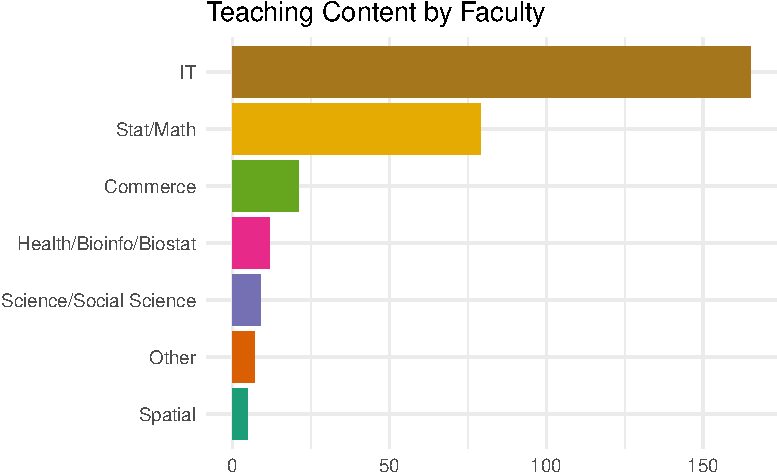
\includegraphics{./03_2-unitext_files/figure-pdf/fig-unitcode-1.pdf}

}

\caption{\label{fig-unitcode}Teaching Content by Faculty}

\end{figure}

Similar findings could be observed from some but not all Go8
universities. Figure~\ref{fig-tile} shows a heat map of the faculty
breakdown by university. Since the total number of units offered by each
university is different, instead of showing the actual number,
proportions are plotted to make better comparisons across universities.

\begin{figure}

{\centering 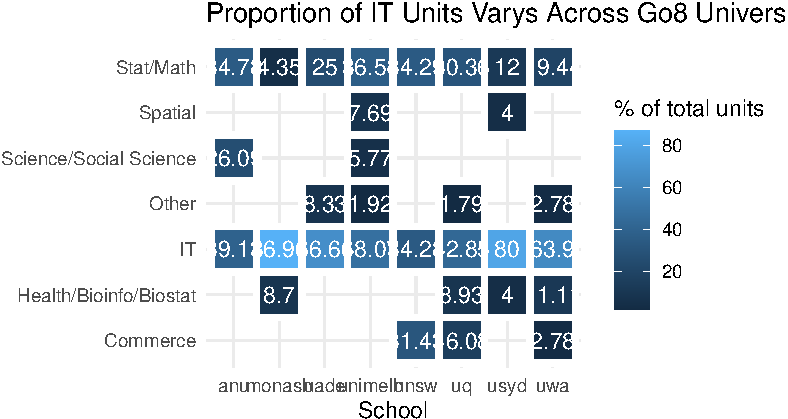
\includegraphics{./03_2-unitext_files/figure-pdf/fig-tile-1.pdf}

}

\caption{\label{fig-tile}Proportion of IT Units Varys Across Go8
Universities}

\end{figure}

Lighter colour represents higher proportion, it is obvious that at
Monash University (monash), University of Adelaide (Uuade), University
of Sydney (usyd) and University of Western Australia (uwa), units from
IT faculty occupies more than 50\% of the total units offered,
especially at Monash University, the proportion of IT units nearly
reaches 87\%.

On the other hand, University of Melbourne (unimelb) and University of
Queensland (uq) offers relatively higher proportion of statistical and
mathematical (Stat/Math) units, almost the same percentage as IT units.
Whereas units offered at the Australian National University (anu) and
UNSW Sydney (unsw) are more evenly distributed across IT, Stat/Math,
Science/Social Science and Commerce respectively.

In addition, it is also clear that units offered at University of
Melbourne (unimelb), University of Queensland (uq) and University of
Western Australia (uwa) covers five out of eight categories, which
implies the Master of Data Science degrees at these three universities
provide more varieties in terms of units offered.

Based on the findings above, it seems that there is a shared structure
across Go8 that Master of Data Science is a IT based, computational
degree, but the proportion it occupies varies by universities. Monash
University tends to be heavily focused on IT and computational aspects,
whereas the Master of Data Science degree at UNSW Sydney and ANU are
more balanced across IT, statistics and math, as well as science and
commerce.

\hypertarget{sec-unit-bigram}{%
\section{Unit Overview and Learning Outcome -
Bigram}\label{sec-unit-bigram}}

After having a rough idea of the bigger picture, we then moved to
explore what exactly are the teaching contents. We pre-processed text
from learning outcome and unit overview to produce single word analysis,
bigram, and tirgram. Words and terms such as `student', `successful
completion' add more noises than values to the results, are removed in
the pre-processing step.

The bigram, shown in Figure~\ref{fig-bigram} below provides the most
informative results among the n-gram analysis. Machine learning (machin
learn) appears quite often, as well as software development (softwar
develop), linear model, statistical analysis (statist analysi), spatial
data. It seems that these frequently mentioned terms are associated with
both computational and statistical concepts and skills, which aligns
with the findings from the unit code analysis in previous section.

\begin{figure}

{\centering 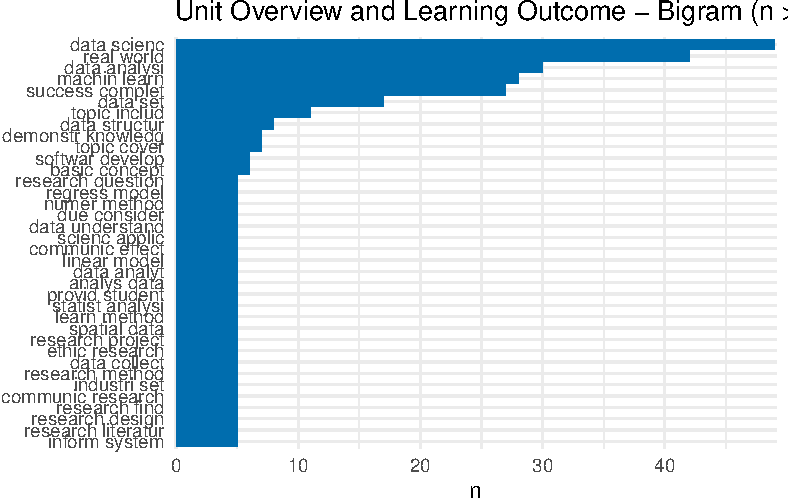
\includegraphics{./03_2-unitext_files/figure-pdf/fig-bigram-1.pdf}

}

\caption{\label{fig-bigram}Unit Overview and Learning Outcome - Bigram
(n \textgreater{} 4)}

\end{figure}

Unfortunately, due to the limited number of observations in the
collected data set, the count for each term is too low to make
meaningful interpretations or justifications. In addition, similar terms
such as research findings, research designs and research literature are
supposed to be grouped and counted together, but are not in the bigram.
This issue is later solved by introducing the topic modeling technique
for natural language processing, which will be discussed in Topic
Modelling section.

\hypertarget{sec-job-analysis}{%
\chapter{Job Text Analysis}\label{sec-job-analysis}}

To explore the skills and programming languages in demand from
employers, we focused on the mobileAdTemplate and the 25 columns of
programming languages. The variable mobileAdtemplate contains the job
description for the position. Using this variable, we conducted text
analysis and produced plots for single word frequencies, bigram, and
trigram.

\hypertarget{sec-word-frequency}{%
\section{Word Frequency}\label{sec-word-frequency}}

\begin{figure}

{\centering 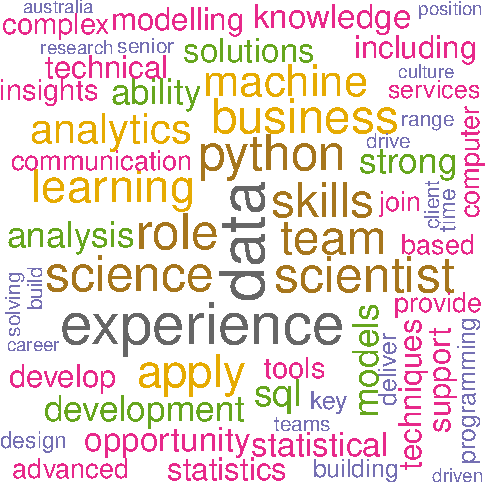
\includegraphics{./03_3-jobtext_files/figure-pdf/fig-job-freqency-1.pdf}

}

\caption{\label{fig-job-freqency}Job Word Frequency (freq
\textgreater200)}

\end{figure}

Word frequency was calculated using the same method as
Section~\ref{sec-unit-bigram}. Programming languages Python and SQL
seems prominent. Potentially due to the amount of senior positions in
the data, \emph{experience} is mentioned a lot. In terms of other
knowledge or skills, \emph{statistics}, \emph{modelling},
\emph{analysis} are some terms that seems to be standing out. To ensure
frequency is meaningful, we looked at bigram and trigram.

\hypertarget{bigram}{%
\section{Bigram}\label{bigram}}

\begin{figure}

{\centering 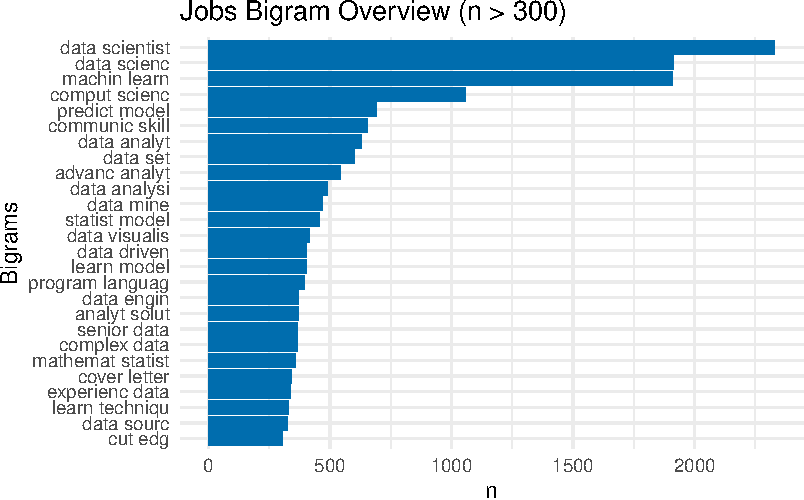
\includegraphics{./03_3-jobtext_files/figure-pdf/fig-employer-bigram-1.pdf}

}

\caption{\label{fig-employer-bigram}Job Description - Bigram (n
\textgreater{} 300}

\end{figure}

For Figure~\ref{fig-employer-bigram}, we stemmed the words before
joining them into bigram in attempt to avoid under-counting. However,
from the figure we can still see that some terms like \emph{data analyt}
and \emph{data analysi} are still counted separately. From this bigram,
the popular skills or knowledge mentioned are \emph{machin learn},
\emph{predict model}, \emph{communic skill}, \emph{data analyt} and
\emph{data mine}. Mathematical skill, \emph{mathemat statist} is also
mentioned quite often. Some of these terms on the list are vague and can
mean be grouped together. Trigram yielded similar results as the bigram.
With the same problem of under-counting the n-grams due to insufficient
groupings.

\hypertarget{programming-languages}{%
\section{Programming Languages}\label{programming-languages}}

\begin{figure}

{\centering 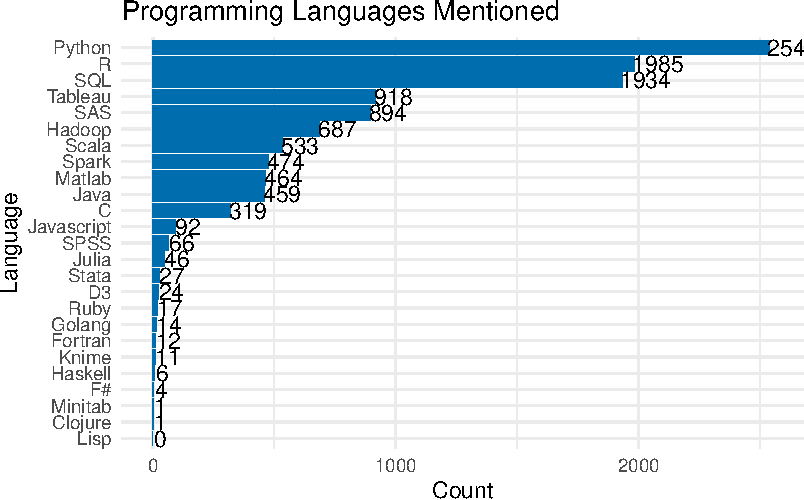
\includegraphics{./03_3-jobtext_files/figure-pdf/fig-languages-1.pdf}

}

\caption{\label{fig-languages}Programming Skills Mentioned by Employers}

\end{figure}

Figure~\ref{fig-languages} shows the count of each language mentioned by
employers. 89\% of the jobs mentioned Python, 69\% mentioned R and 68\%
mentioned SQL. Tableau's popularity is not a surprise given the high
frequency for \emph{data visualis} in the previous section.

\part{Topic Modelling}

As mentioned in Section Section~\ref{sec-unit-bigram}, since the
collected university data is relatively small, to make more educated and
meaningful interpretations, similar words shall be grouped together and
counted by groups. This is usually computed using text corpus, which is
a language resource consisting of a large and structured set of texts,
since data science is a new term waiting to be defined, there is no
available text corpus on this topic. Therefore, we adopted the concept
of word embedding models and tried to build our own text corpus.

There are multiple publicly available models and packages to conduct
similar computations, such as \texttt{word2vec} and \texttt{text2vec},
however, each model takes hours to fit. Due to time constrains, we have
only fitted the Dirichlet Allocation (LDA) model with a few parameter
adjustments using the \texttt{text2vec} package with the concepts
illustrated by Das (2016).

\hypertarget{sec-model}{%
\section*{Algorithm and Model Fitting}\label{sec-model}}
\addcontentsline{toc}{section}{Algorithm and Model Fitting}

According to Das (2016), the algorithm behind the LDA model is to
convert words to document-term matrix (DTM), where the rows, columns and
entries correspond to documents, terms and counts respectively. LDA then
fits a probabilistic model that assumes a mixture of latent topics,
where each topic has a multinomial distribution for all words. The
number of topics is a parameter that could be adjusted by needs.

The model must be trained before it could be used, we web scraped 4448
Wikipedia articles as training data, including 2816 articles in
statistics, 1005 articles in sociology and 627 in computing. The initial
codes and functions to build the LDA model was provided by Dr Tanaka, we
have tested model outputs using different number of topics and tried out
training the LDA models with different combinations of data.

The table below shows a glimpse of the model output of the initial LDA
model, after training by data collected from all 4448 Wikipedia articles
on 12 topics.

\begin{table}
\centering
\resizebox{\linewidth}{!}{
\begin{tabular}{c|c|c}
\hline
topic & term & beta\\
\hline
\cellcolor{gray!6}{1} & \cellcolor{gray!6}{abov\_mention} & \cellcolor{gray!6}{3.30e-06}\\
\hline
2 & abov\_mention & 2.30e-06\\
\hline
\cellcolor{gray!6}{3} & \cellcolor{gray!6}{abov\_mention} & \cellcolor{gray!6}{8.70e-06}\\
\hline
4 & abov\_mention & 1.79e-05\\
\hline
\cellcolor{gray!6}{5} & \cellcolor{gray!6}{abov\_mention} & \cellcolor{gray!6}{2.00e-07}\\
\hline
\end{tabular}}
\end{table}

Term shows all the word extracted from the training data (Wikipedia
articles), as each latent topic has a multinomial distribution for all
words, beta value of a term is the score / probability computed for that
particular topic. Highest beta value indicates highest probability,
which means the term is most likely belongs to the corresponding topic.

Beta values for the same word would differ from model to model, and also
subject to change by adjusting the number of latent topics. To acquire
the most satisfactory results for our university data, we have fitted
and tested multiple LDA models with different subset of training data,
as well as various number of topics.

\hypertarget{model-adjustments}{%
\section*{Model Adjustments}\label{model-adjustments}}
\addcontentsline{toc}{section}{Model Adjustments}

After applying the fitted LDA models to our university data set, the
results delivered by the models are quite different.
Figure~\ref{fig-com} compares the results produced by the four fitted
models using different training data on ten topics.

\begin{figure}

{\centering 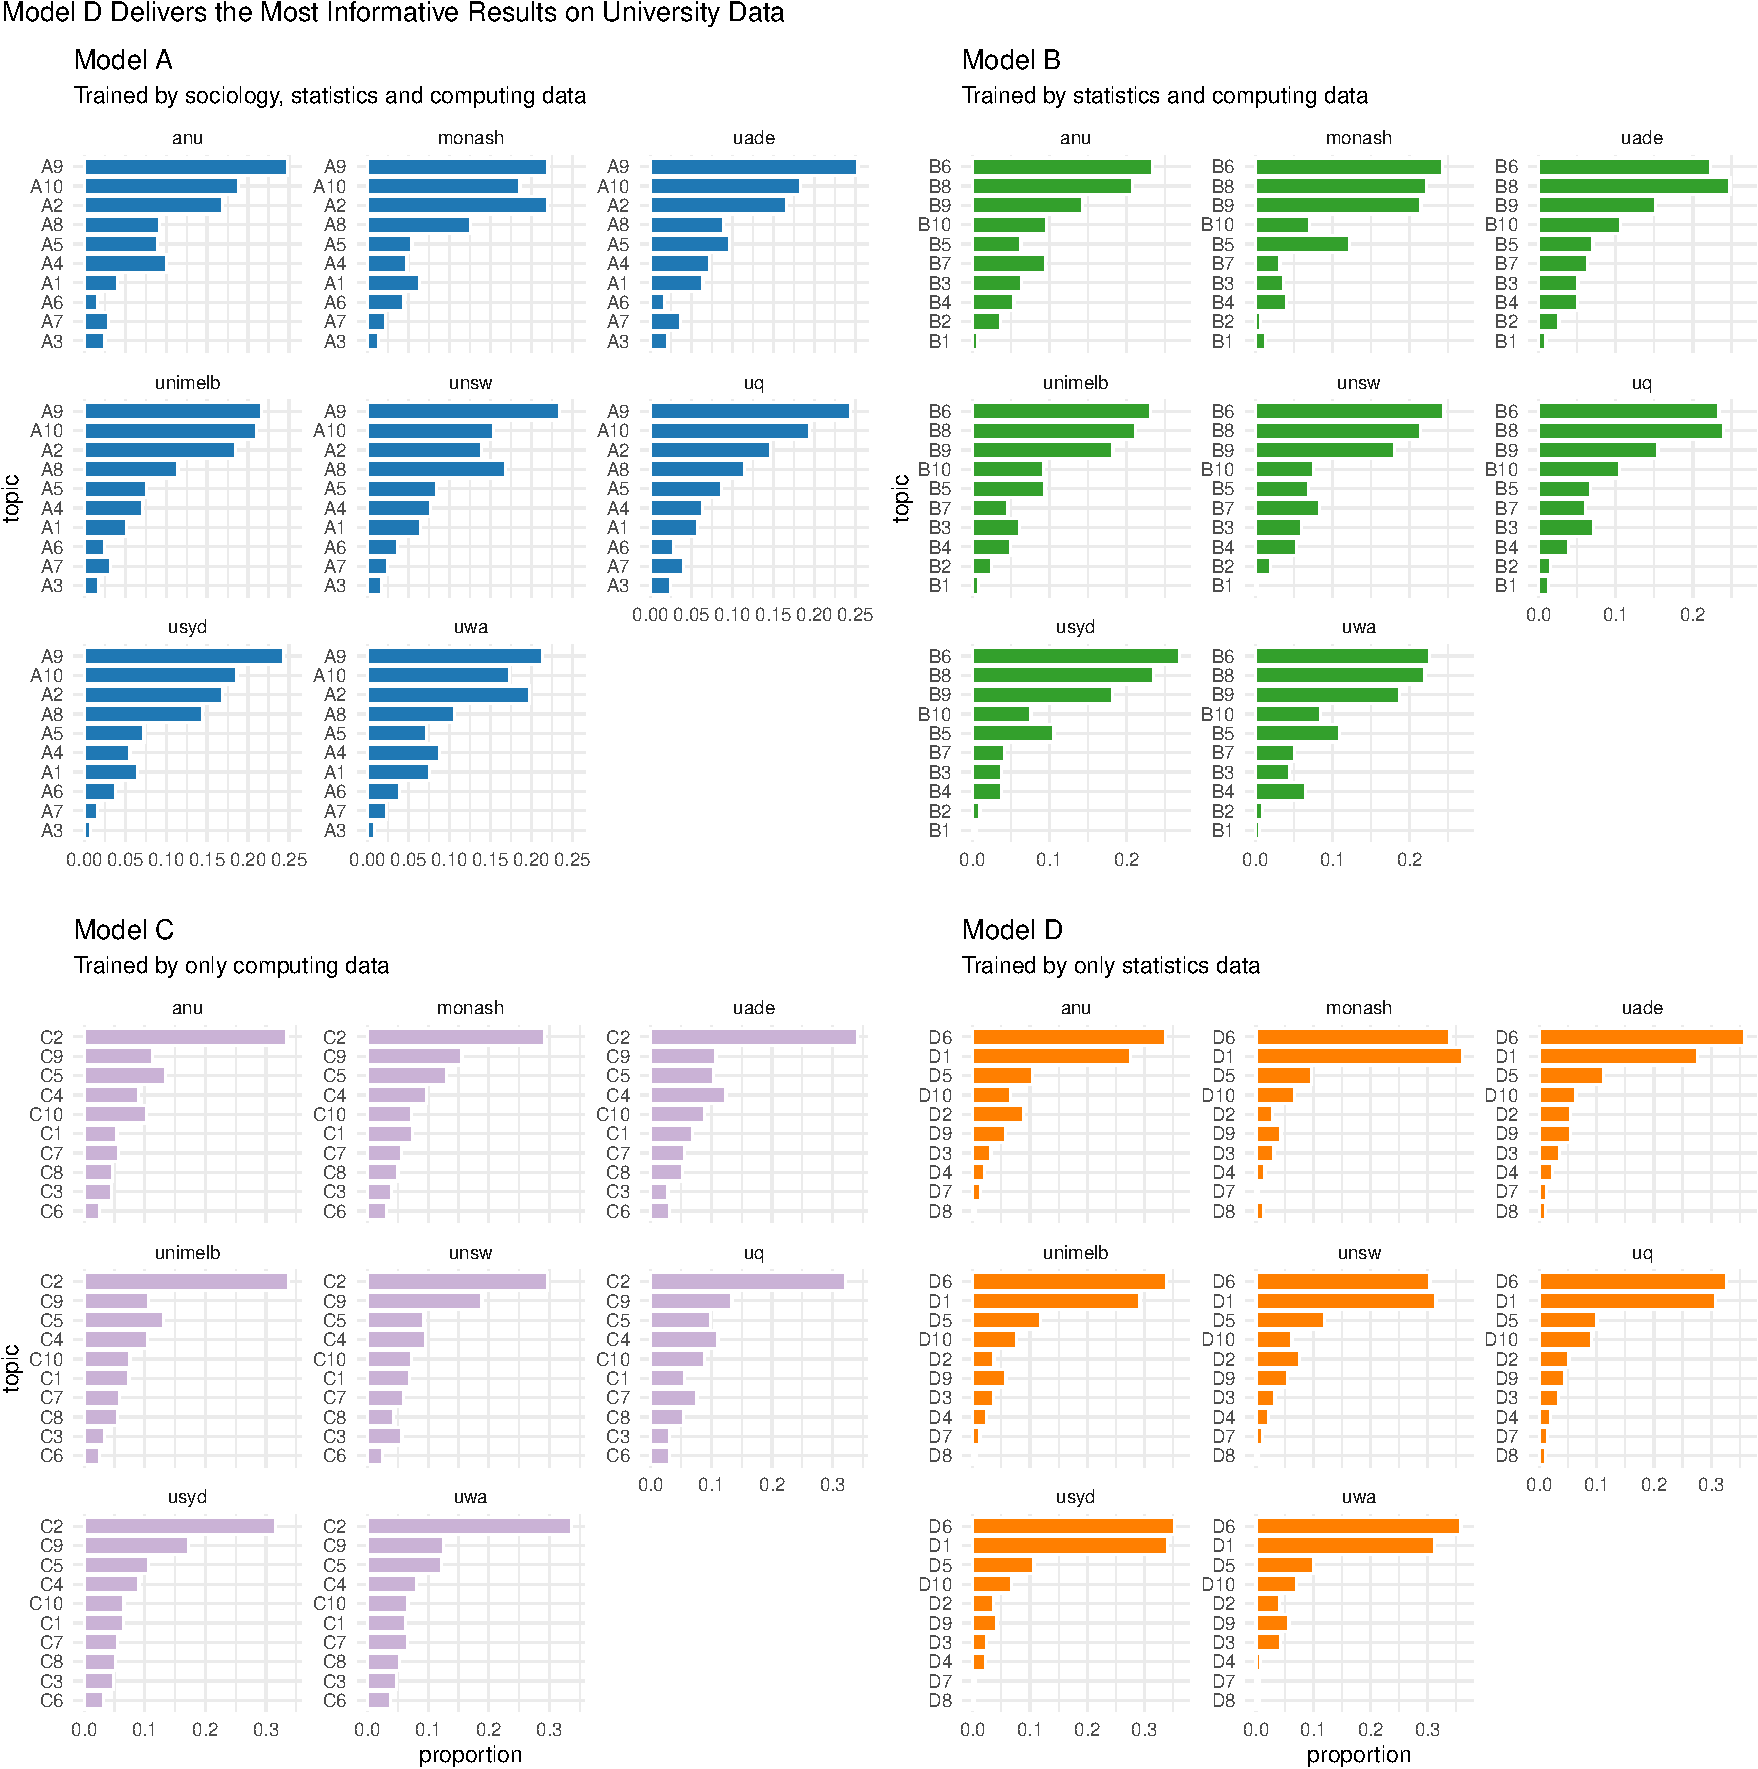
\includegraphics{./04-text2vec_files/figure-pdf/fig-com-1.pdf}

}

\caption{\label{fig-com}Model D Delivers the Most Informative Results on
University Data}

\end{figure}

For Model A, Topics A9, A10, A2 and A8 occupies relatively higher
proportion compare with the others, but the order varies across
universities, and their proportions are not significantly larger than
the rest of other topics, makes it hard to draw meaningful
interpretations. On the top right, Model B demonstrates a better
picture: Topics B6, B8 and B9 are the top 3 topics across all Go8
universities, however, proportions of Topics B10, B5, B7, B3 and B4 are
also obvious higher in some of the universities, brings in difficulties
to make justifications.

As sociology data tends to brings in noises to the model, and is not
closely relevant to the data science topic compare with statistics and
computing, Model C and D are fitted using only statistics data and
computing data respectively. Topic C2 is the only dominating topic in
Model C, where as Topics D6 and D1 occupy significantly large proportion
in Model D. Besides, cccccc together took a relatively higher proportion
compare with the rest of other topics in Model D.

The table below listed the top 30 words of each topics in Model C, it
turns out Topic C2 contains words like comput (computation,
computational, computer), system, program, machin (machine), softwar
(software), model, test, calcul (calculate, calculation) and data, which
seems to be associated with mainly computational aspects.

\begin{table}
\centering
\begin{tabular}{l|l|l|l|l|l|l|l|l|l}
\hline
Topic C1 & Topic C2 & Topic C3 & Topic C4 & Topic C5 & Topic C6 & Topic C7 & Topic C8 & Topic C9 & Topic C10\\
\hline
window & comput & ibm & algorithm & network & bit & format & intel & softwar & languag\\
\hline
system & system & comput & can & use & instruct & use & chip & compani & program\\
\hline
version & program & system & number & can & memori & imag & design & appl & use\\
\hline
releas & use & disk & function & web & use & digit & processor & free & compil\\
\hline
support & machin & drive & set & data & address & can & bit & use & code\\
\hline
user & design & use & state & internet & regist & video & core & also & function\\
\hline
oper\_system & process & control & languag & secur & processor & standard & mhz & develop & object\\
\hline
oper & develop & machin & use & access & oper & disc & use & open & type\\
\hline
os & inform & card & symbol & protocol & can & data & introduc & sourc & can\\
\hline
file & softwar & unit & problem & link & data & file & microprocessor & user & implement\\
\hline
microsoft & engin & amiga & grammar & connect & system & encod & technolog & aol & program\_languag\\
\hline
use & first & pc & rule & server & page & dvd & motorola & public & standard\\
\hline
applic & time & model & parser & servic & mode & edit & clock & state & charact\\
\hline
includ & research & storag & recurs & standard & architectur & pdf & power & new & exampl\\
\hline
develop & can & data & one & devic & also & code & ghz & hacker & class\\
\hline
unix & logic & commodor & input & node & set & cd & bus & project & also\\
\hline
mac & scienc & home & exampl & communic & one & camera & cpu & includ & name\\
\hline
command & work & hardwar & machin & provid & code & audio & generat & year & call\\
\hline
interfac & model & game & ture & attack & access & compress & perform & licens & line\\
\hline
also & oper & one & comput & may & byte & ray & support & law & variabl\\
\hline
dos & perform & oper & two & key & onli & also & seri & product & data\\
\hline
server & one & time & follow & also & program & includ & base & us & list\\
\hline
featur & test & atari & ani & client & comput & blu & product & open\_sourc & includ\\
\hline
appl & calcul & ii & pars & system & execut & blu\_ray & model & free\_softwar & java\\
\hline
run & data & tape & context & browser & cpu & graphic & first & game & statement\\
\hline
base & univers & graphic & time & user & store & allow & cach & servic & valu\\
\hline
shell & mani & market & defin & page & point & print & market & busi & develop\\
\hline
linux & human & product & express & messag & number & media & two & technolog & interpret\\
\hline
manag & electron & display & string & applic & unit & store & famili & announc & structur\\
\hline
new & method & cp & onli & ethernet & perform & record & mb & work & support\\
\hline
\end{tabular}
\end{table}

Although Model D provides a reasonably meaningful result, there is not
much interpretations could be made for the other topics, the information
it offers is still not very satisfying. Compares with Model C, Model D
has two domination topics D6 and D1, topics D5, D10, D2, D9 also
accounts for a large proportion, which together provides more
information. Therefore, Model D, which is trained by only statistics
data on ten topics, is selected to use for further analysis on our
university data.

Note that it requires highly skilled linguists and huge efforts to
establish a proper text corpus, the model we built is still fairly basic
and could be further optimised by adjustments.

\hypertarget{sec-unitopic}{%
\chapter{Apply the Selected Model to Collected University
Data}\label{sec-unitopic}}

Before applying the fitted LDA model to our university data set, words
from unit overview and learning outcomes are stemmed using the
\texttt{SnowballC} package, so that noises like plurals and part of
speech are removed. The stemmed words are then assigned to the
corresponding topic with the highest beta score, as explained in Section
\textbf{?@sec-model}. Instead of counting the appearance of words, the
new counts generated are based on topics.

Similar with the university breakdown in Section~\ref{sec-unit-bigram},
to make more objective comparisons, counts are converted to proportions
due to different number of units scraped for the eight universities.
Figure~\ref{fig-unitopics} suggests that Topics 1 and 6 are obviously
the dominating topics in Master of data science at all Go8 universities,
whereas Topics 2, 5, 9, 10 together also occupies a relatively large
proportion.

\begin{figure}

{\centering 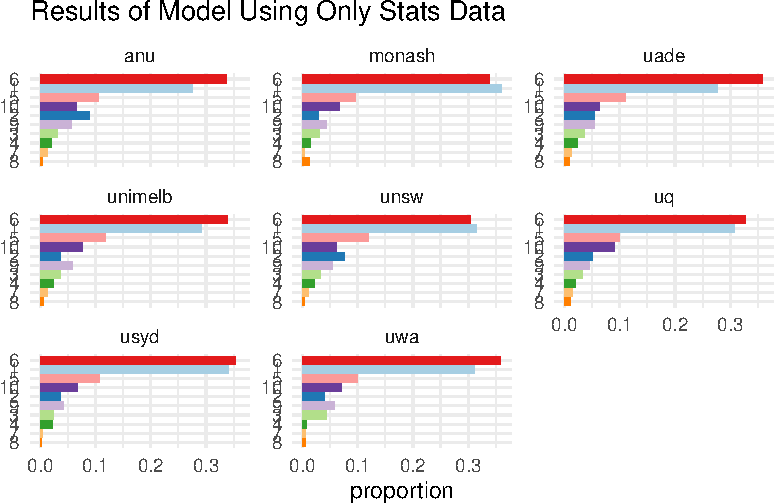
\includegraphics{./04_1-unilda_files/figure-pdf/fig-unitopics-1.pdf}

}

\caption{\label{fig-unitopics}Topics Proportion by University}

\end{figure}

The top 30 words based on probabilities for each of the ten topics are
provided below, colours of the columns are aligned with
Figure~\ref{fig-unitopics}. Topic 1 contains words like statist
(statistics), data, popul (population), system, bias, experiment, and we
can see data, algorithm, analysi (analysis), model, cluster, comput
(computation, computer, computational), function, spatial in topic 6, it
is a reasonable interpretation that these two topics are both associated
with computational aspects.

\begin{figure}

{\centering 

\hypertarget{fig-topics-1}{}
\begin{table}
\centering\begingroup\fontsize{12}{14}\selectfont

\begin{tabular}{>{}l|>{}l|>{}l|>{}l|>{}l|>{}l|>{}l|>{}l|>{}l|>{}l}
\hline
Topic 1 & Topic 2 & Topic 3 & Topic 4 & Topic 5 & Topic 6 & Topic 7 & Topic 8 & Topic 9 & Topic 10\\
\hline
\cellcolor[HTML]{A6CEE3}{\textcolor{white}{studi}} & \cellcolor[HTML]{1F78B4}{\textcolor{white}{model}} & \cellcolor[HTML]{B2DF8A}{\textcolor{white}{sampl}} & \cellcolor[HTML]{33A02C}{\textcolor{white}{theta}} & \cellcolor[HTML]{FB9A99}{\textcolor{white}{probabl}} & \cellcolor[HTML]{E31A1C}{\textcolor{white}{data}} & \cellcolor[HTML]{FDBF6F}{\textcolor{white}{distribut}} & \cellcolor[HTML]{FF7F00}{\textcolor{white}{x\_}} & \cellcolor[HTML]{CAB2D6}{\textcolor{white}{test}} & \cellcolor[HTML]{6A3D9A}{\textcolor{white}{process}}\\
\hline
\cellcolor[HTML]{A6CEE3}{\textcolor{white}{use}} & \cellcolor[HTML]{1F78B4}{\textcolor{white}{variabl}} & \cellcolor[HTML]{B2DF8A}{\textcolor{white}{estim}} & \cellcolor[HTML]{33A02C}{\textcolor{white}{function}} & \cellcolor[HTML]{FB9A99}{\textcolor{white}{one}} & \cellcolor[HTML]{E31A1C}{\textcolor{white}{use}} & \cellcolor[HTML]{FDBF6F}{\textcolor{white}{frac}} & \cellcolor[HTML]{FF7F00}{\textcolor{white}{frac}} & \cellcolor[HTML]{CAB2D6}{\textcolor{white}{statist}} & \cellcolor[HTML]{6A3D9A}{\textcolor{white}{time}}\\
\hline
\cellcolor[HTML]{A6CEE3}{\textcolor{white}{statist}} & \cellcolor[HTML]{1F78B4}{\textcolor{white}{regress}} & \cellcolor[HTML]{B2DF8A}{\textcolor{white}{mean}} & \cellcolor[HTML]{33A02C}{\textcolor{white}{probabl}} & \cellcolor[HTML]{FB9A99}{\textcolor{white}{number}} & \cellcolor[HTML]{E31A1C}{\textcolor{white}{algorithm}} & \cellcolor[HTML]{FDBF6F}{\textcolor{white}{alpha}} & \cellcolor[HTML]{FF7F00}{\textcolor{white}{left}} & \cellcolor[HTML]{CAB2D6}{\textcolor{white}{hypothesi}} & \cellcolor[HTML]{6A3D9A}{\textcolor{white}{point}}\\
\hline
\cellcolor[HTML]{A6CEE3}{\textcolor{white}{research}} & \cellcolor[HTML]{1F78B4}{\textcolor{white}{estim}} & \cellcolor[HTML]{B2DF8A}{\textcolor{white}{valu}} & \cellcolor[HTML]{33A02C}{\textcolor{white}{x\_x}} & \cellcolor[HTML]{FB9A99}{\textcolor{white}{theori}} & \cellcolor[HTML]{E31A1C}{\textcolor{white}{analysi}} & \cellcolor[HTML]{FDBF6F}{\textcolor{white}{mu}} & \cellcolor[HTML]{FF7F00}{\textcolor{white}{right}} & \cellcolor[HTML]{CAB2D6}{\textcolor{white}{valu}} & \cellcolor[HTML]{6A3D9A}{\textcolor{white}{stochast}}\\
\hline
\cellcolor[HTML]{A6CEE3}{\textcolor{white}{data}} & \cellcolor[HTML]{1F78B4}{\textcolor{white}{beta}} & \cellcolor[HTML]{B2DF8A}{\textcolor{white}{distribut}} & \cellcolor[HTML]{33A02C}{\textcolor{white}{distribut}} & \cellcolor[HTML]{FB9A99}{\textcolor{white}{bayesian}} & \cellcolor[HTML]{E31A1C}{\textcolor{white}{can}} & \cellcolor[HTML]{FDBF6F}{\textcolor{white}{beta}} & \cellcolor[HTML]{FF7F00}{\textcolor{white}{sum}} & \cellcolor[HTML]{CAB2D6}{\textcolor{white}{two}} & \cellcolor[HTML]{6A3D9A}{\textcolor{white}{state}}\\
\hline
\cellcolor[HTML]{A6CEE3}{\textcolor{white}{design}} & \cellcolor[HTML]{1F78B4}{\textcolor{white}{linear}} & \cellcolor[HTML]{B2DF8A}{\textcolor{white}{varianc}} & \cellcolor[HTML]{33A02C}{\textcolor{white}{variabl}} & \cellcolor[HTML]{FB9A99}{\textcolor{white}{event}} & \cellcolor[HTML]{E31A1C}{\textcolor{white}{method}} & \cellcolor[HTML]{FDBF6F}{\textcolor{white}{function}} & \cellcolor[HTML]{FF7F00}{\textcolor{white}{operatornam}} & \cellcolor[HTML]{CAB2D6}{\textcolor{white}{number}} & \cellcolor[HTML]{6A3D9A}{\textcolor{white}{function}}\\
\hline
\cellcolor[HTML]{A6CEE3}{\textcolor{white}{can}} & \cellcolor[HTML]{1F78B4}{\textcolor{white}{use}} & \cellcolor[HTML]{B2DF8A}{\textcolor{white}{statist}} & \cellcolor[HTML]{33A02C}{\textcolor{white}{random}} & \cellcolor[HTML]{FB9A99}{\textcolor{white}{can}} & \cellcolor[HTML]{E31A1C}{\textcolor{white}{model}} & \cellcolor[HTML]{FDBF6F}{\textcolor{white}{gamma}} & \cellcolor[HTML]{FF7F00}{\textcolor{white}{sigma}} & \cellcolor[HTML]{CAB2D6}{\textcolor{white}{use}} & \cellcolor[HTML]{6A3D9A}{\textcolor{white}{can}}\\
\hline
\cellcolor[HTML]{A6CEE3}{\textcolor{white}{effect}} & \cellcolor[HTML]{1F78B4}{\textcolor{white}{y\_}} & \cellcolor[HTML]{B2DF8A}{\textcolor{white}{use}} & \cellcolor[HTML]{33A02C}{\textcolor{white}{x\_}} & \cellcolor[HTML]{FB9A99}{\textcolor{white}{prior}} & \cellcolor[HTML]{E31A1C}{\textcolor{white}{set}} & \cellcolor[HTML]{FDBF6F}{\textcolor{white}{right}} & \cellcolor[HTML]{FF7F00}{\textcolor{white}{y\_}} & \cellcolor[HTML]{CAB2D6}{\textcolor{white}{correl}} & \cellcolor[HTML]{6A3D9A}{\textcolor{white}{random}}\\
\hline
\cellcolor[HTML]{A6CEE3}{\textcolor{white}{popul}} & \cellcolor[HTML]{1F78B4}{\textcolor{white}{squar}} & \cellcolor[HTML]{B2DF8A}{\textcolor{white}{standard}} & \cellcolor[HTML]{33A02C}{\textcolor{white}{random\_variabl}} & \cellcolor[HTML]{FB9A99}{\textcolor{white}{infer}} & \cellcolor[HTML]{E31A1C}{\textcolor{white}{cluster}} & \cellcolor[HTML]{FDBF6F}{\textcolor{white}{left}} & \cellcolor[HTML]{FF7F00}{\textcolor{white}{cdot}} & \cellcolor[HTML]{CAB2D6}{\textcolor{white}{rank}} & \cellcolor[HTML]{6A3D9A}{\textcolor{white}{markov}}\\
\hline
\cellcolor[HTML]{A6CEE3}{\textcolor{white}{may}} & \cellcolor[HTML]{1F78B4}{\textcolor{white}{can}} & \cellcolor[HTML]{B2DF8A}{\textcolor{white}{popul}} & \cellcolor[HTML]{33A02C}{\textcolor{white}{mathcal}} & \cellcolor[HTML]{FB9A99}{\textcolor{white}{use}} & \cellcolor[HTML]{E31A1C}{\textcolor{white}{comput}} & \cellcolor[HTML]{FDBF6F}{\textcolor{white}{normal}} & \cellcolor[HTML]{FF7F00}{\textcolor{white}{operatornam\_e}} & \cellcolor[HTML]{CAB2D6}{\textcolor{white}{measur}} & \cellcolor[HTML]{6A3D9A}{\textcolor{white}{space}}\\
\hline
\cellcolor[HTML]{A6CEE3}{\textcolor{white}{control}} & \cellcolor[HTML]{1F78B4}{\textcolor{white}{depend}} & \cellcolor[HTML]{B2DF8A}{\textcolor{white}{deviat}} & \cellcolor[HTML]{33A02C}{\textcolor{white}{p\_x}} & \cellcolor[HTML]{FB9A99}{\textcolor{white}{exampl}} & \cellcolor[HTML]{E31A1C}{\textcolor{white}{point}} & \cellcolor[HTML]{FDBF6F}{\textcolor{white}{lambda}} & \cellcolor[HTML]{FF7F00}{\textcolor{white}{matrix}} & \cellcolor[HTML]{CAB2D6}{\textcolor{white}{differ}} & \cellcolor[HTML]{6A3D9A}{\textcolor{white}{system}}\\
\hline
\cellcolor[HTML]{A6CEE3}{\textcolor{white}{experi}} & \cellcolor[HTML]{1F78B4}{\textcolor{white}{data}} & \cellcolor[HTML]{B2DF8A}{\textcolor{white}{data}} & \cellcolor[HTML]{33A02C}{\textcolor{white}{mid}} & \cellcolor[HTML]{FB9A99}{\textcolor{white}{random}} & \cellcolor[HTML]{E31A1C}{\textcolor{white}{function}} & \cellcolor[HTML]{FDBF6F}{\textcolor{white}{paramet}} & \cellcolor[HTML]{FF7F00}{\textcolor{white}{xi}} & \cellcolor[HTML]{CAB2D6}{\textcolor{white}{signific}} & \cellcolor[HTML]{6A3D9A}{\textcolor{white}{textstyl}}\\
\hline
\cellcolor[HTML]{A6CEE3}{\textcolor{white}{analysi}} & \cellcolor[HTML]{1F78B4}{\textcolor{white}{valu}} & \cellcolor[HTML]{B2DF8A}{\textcolor{white}{error}} & \cellcolor[HTML]{33A02C}{\textcolor{white}{likelihood}} & \cellcolor[HTML]{FB9A99}{\textcolor{white}{given}} & \cellcolor[HTML]{E31A1C}{\textcolor{white}{learn}} & \cellcolor[HTML]{FDBF6F}{\textcolor{white}{sigma}} & \cellcolor[HTML]{FF7F00}{\textcolor{white}{e⁡}} & \cellcolor[HTML]{CAB2D6}{\textcolor{white}{posit}} & \cellcolor[HTML]{6A3D9A}{\textcolor{white}{use}}\\
\hline
\cellcolor[HTML]{A6CEE3}{\textcolor{white}{also}} & \cellcolor[HTML]{1F78B4}{\textcolor{white}{error}} & \cellcolor[HTML]{B2DF8A}{\textcolor{white}{interv}} & \cellcolor[HTML]{33A02C}{\textcolor{white}{f\_x}} & \cellcolor[HTML]{FB9A99}{\textcolor{white}{statist}} & \cellcolor[HTML]{E31A1C}{\textcolor{white}{also}} & \cellcolor[HTML]{FDBF6F}{\textcolor{white}{nu}} & \cellcolor[HTML]{FF7F00}{\textcolor{white}{mu}} & \cellcolor[HTML]{CAB2D6}{\textcolor{white}{one}} & \cellcolor[HTML]{6A3D9A}{\textcolor{white}{signal}}\\
\hline
\cellcolor[HTML]{A6CEE3}{\textcolor{white}{differ}} & \cellcolor[HTML]{1F78B4}{\textcolor{white}{effect}} & \cellcolor[HTML]{B2DF8A}{\textcolor{white}{can}} & \cellcolor[HTML]{33A02C}{\textcolor{white}{valu}} & \cellcolor[HTML]{FB9A99}{\textcolor{white}{problem}} & \cellcolor[HTML]{E31A1C}{\textcolor{white}{base}} & \cellcolor[HTML]{FDBF6F}{\textcolor{white}{sqrt}} & \cellcolor[HTML]{FF7F00}{\textcolor{white}{hat}} & \cellcolor[HTML]{CAB2D6}{\textcolor{white}{score}} & \cellcolor[HTML]{6A3D9A}{\textcolor{white}{measur}}\\
\hline
\cellcolor[HTML]{A6CEE3}{\textcolor{white}{measur}} & \cellcolor[HTML]{1F78B4}{\textcolor{white}{independ}} & \cellcolor[HTML]{B2DF8A}{\textcolor{white}{median}} & \cellcolor[HTML]{33A02C}{\textcolor{white}{f\_}} & \cellcolor[HTML]{FB9A99}{\textcolor{white}{valu}} & \cellcolor[HTML]{E31A1C}{\textcolor{white}{distanc}} & \cellcolor[HTML]{FDBF6F}{\textcolor{white}{normal\_distribut}} & \cellcolor[HTML]{FF7F00}{\textcolor{white}{end}} & \cellcolor[HTML]{CAB2D6}{\textcolor{white}{null}} & \cellcolor[HTML]{6A3D9A}{\textcolor{white}{t\_t}}\\
\hline
\cellcolor[HTML]{A6CEE3}{\textcolor{white}{group}} & \cellcolor[HTML]{1F78B4}{\textcolor{white}{fit}} & \cellcolor[HTML]{B2DF8A}{\textcolor{white}{measur}} & \cellcolor[HTML]{33A02C}{\textcolor{white}{measur}} & \cellcolor[HTML]{FB9A99}{\textcolor{white}{decis}} & \cellcolor[HTML]{E31A1C}{\textcolor{white}{problem}} & \cellcolor[HTML]{FDBF6F}{\textcolor{white}{log}} & \cellcolor[HTML]{FF7F00}{\textcolor{white}{begin}} & \cellcolor[HTML]{CAB2D6}{\textcolor{white}{ratio}} & \cellcolor[HTML]{6A3D9A}{\textcolor{white}{one}}\\
\hline
\cellcolor[HTML]{A6CEE3}{\textcolor{white}{exampl}} & \cellcolor[HTML]{1F78B4}{\textcolor{white}{paramet}} & \cellcolor[HTML]{B2DF8A}{\textcolor{white}{normal}} & \cellcolor[HTML]{33A02C}{\textcolor{white}{leq}} & \cellcolor[HTML]{FB9A99}{\textcolor{white}{expect}} & \cellcolor[HTML]{E31A1C}{\textcolor{white}{one}} & \cellcolor[HTML]{FDBF6F}{\textcolor{white}{ln}} & \cellcolor[HTML]{FF7F00}{\textcolor{white}{align}} & \cellcolor[HTML]{CAB2D6}{\textcolor{white}{group}} & \cellcolor[HTML]{6A3D9A}{\textcolor{white}{number}}\\
\hline
\cellcolor[HTML]{A6CEE3}{\textcolor{white}{treatment}} & \cellcolor[HTML]{1F78B4}{\textcolor{white}{observ}} & \cellcolor[HTML]{B2DF8A}{\textcolor{white}{bar}} & \cellcolor[HTML]{33A02C}{\textcolor{white}{log}} & \cellcolor[HTML]{FB9A99}{\textcolor{white}{two}} & \cellcolor[HTML]{E31A1C}{\textcolor{white}{factor}} & \cellcolor[HTML]{FDBF6F}{\textcolor{white}{probabl}} & \cellcolor[HTML]{FF7F00}{\textcolor{white}{covari}} & \cellcolor[HTML]{CAB2D6}{\textcolor{white}{can}} & \cellcolor[HTML]{6A3D9A}{\textcolor{white}{lambda}}\\
\hline
\cellcolor[HTML]{A6CEE3}{\textcolor{white}{result}} & \cellcolor[HTML]{1F78B4}{\textcolor{white}{analysi}} & \cellcolor[HTML]{B2DF8A}{\textcolor{white}{size}} & \cellcolor[HTML]{33A02C}{\textcolor{white}{set}} & \cellcolor[HTML]{FB9A99}{\textcolor{white}{observ}} & \cellcolor[HTML]{E31A1C}{\textcolor{white}{map}} & \cellcolor[HTML]{FDBF6F}{\textcolor{white}{sim}} & \cellcolor[HTML]{FF7F00}{\textcolor{white}{var}} & \cellcolor[HTML]{CAB2D6}{\textcolor{white}{null\_hypothesi}} & \cellcolor[HTML]{6A3D9A}{\textcolor{white}{equat}}\\
\hline
\cellcolor[HTML]{A6CEE3}{\textcolor{white}{time}} & \cellcolor[HTML]{1F78B4}{\textcolor{white}{least}} & \cellcolor[HTML]{B2DF8A}{\textcolor{white}{one}} & \cellcolor[HTML]{33A02C}{\textcolor{white}{x\_y}} & \cellcolor[HTML]{FB9A99}{\textcolor{white}{case}} & \cellcolor[HTML]{E31A1C}{\textcolor{white}{network}} & \cellcolor[HTML]{FDBF6F}{\textcolor{white}{left\_frac}} & \cellcolor[HTML]{FF7F00}{\textcolor{white}{varianc}} & \cellcolor[HTML]{CAB2D6}{\textcolor{white}{coeffici}} & \cellcolor[HTML]{6A3D9A}{\textcolor{white}{also}}\\
\hline
\cellcolor[HTML]{A6CEE3}{\textcolor{white}{includ}} & \cellcolor[HTML]{1F78B4}{\textcolor{white}{function}} & \cellcolor[HTML]{B2DF8A}{\textcolor{white}{standard\_deviat}} & \cellcolor[HTML]{33A02C}{\textcolor{white}{can}} & \cellcolor[HTML]{FB9A99}{\textcolor{white}{model}} & \cellcolor[HTML]{E31A1C}{\textcolor{white}{matrix}} & \cellcolor[HTML]{FDBF6F}{\textcolor{white}{moment}} & \cellcolor[HTML]{FF7F00}{\textcolor{white}{c\_}} & \cellcolor[HTML]{CAB2D6}{\textcolor{white}{negat}} & \cellcolor[HTML]{6A3D9A}{\textcolor{white}{set}}\\
\hline
\cellcolor[HTML]{A6CEE3}{\textcolor{white}{rate}} & \cellcolor[HTML]{1F78B4}{\textcolor{white}{seri}} & \cellcolor[HTML]{B2DF8A}{\textcolor{white}{random}} & \cellcolor[HTML]{33A02C}{\textcolor{white}{xn}} & \cellcolor[HTML]{FB9A99}{\textcolor{white}{law}} & \cellcolor[HTML]{E31A1C}{\textcolor{white}{applic}} & \cellcolor[HTML]{FDBF6F}{\textcolor{white}{cumul}} & \cellcolor[HTML]{FF7F00}{\textcolor{white}{xy}} & \cellcolor[HTML]{CAB2D6}{\textcolor{white}{result}} & \cellcolor[HTML]{6A3D9A}{\textcolor{white}{poisson}}\\
\hline
\cellcolor[HTML]{A6CEE3}{\textcolor{white}{level}} & \cellcolor[HTML]{1F78B4}{\textcolor{white}{equat}} & \cellcolor[HTML]{B2DF8A}{\textcolor{white}{exampl}} & \cellcolor[HTML]{33A02C}{\textcolor{white}{condit}} & \cellcolor[HTML]{FB9A99}{\textcolor{white}{possibl}} & \cellcolor[HTML]{E31A1C}{\textcolor{white}{compon}} & \cellcolor[HTML]{FDBF6F}{\textcolor{white}{densiti}} & \cellcolor[HTML]{FF7F00}{\textcolor{white}{vector}} & \cellcolor[HTML]{CAB2D6}{\textcolor{white}{true}} & \cellcolor[HTML]{6A3D9A}{\textcolor{white}{call}}\\
\hline
\cellcolor[HTML]{A6CEE3}{\textcolor{white}{individu}} & \cellcolor[HTML]{1F78B4}{\textcolor{white}{predict}} & \cellcolor[HTML]{B2DF8A}{\textcolor{white}{confid}} & \cellcolor[HTML]{33A02C}{\textcolor{white}{converg}} & \cellcolor[HTML]{FB9A99}{\textcolor{white}{outcom}} & \cellcolor[HTML]{E31A1C}{\textcolor{white}{similar}} & \cellcolor[HTML]{FDBF6F}{\textcolor{white}{pi}} & \cellcolor[HTML]{FF7F00}{\textcolor{white}{x\_x}} & \cellcolor[HTML]{CAB2D6}{\textcolor{white}{type}} & \cellcolor[HTML]{6A3D9A}{\textcolor{white}{theori}}\\
\hline
\cellcolor[HTML]{A6CEE3}{\textcolor{white}{system}} & \cellcolor[HTML]{1F78B4}{\textcolor{white}{statist}} & \cellcolor[HTML]{B2DF8A}{\textcolor{white}{weight}} & \cellcolor[HTML]{33A02C}{\textcolor{white}{paramet}} & \cellcolor[HTML]{FB9A99}{\textcolor{white}{rule}} & \cellcolor[HTML]{E31A1C}{\textcolor{white}{two}} & \cellcolor[HTML]{FDBF6F}{\textcolor{white}{variabl}} & \cellcolor[HTML]{FF7F00}{\textcolor{white}{n\_}} & \cellcolor[HTML]{CAB2D6}{\textcolor{white}{item}} & \cellcolor[HTML]{6A3D9A}{\textcolor{white}{frequenc}}\\
\hline
\cellcolor[HTML]{A6CEE3}{\textcolor{white}{bias}} & \cellcolor[HTML]{1F78B4}{\textcolor{white}{least\_squar}} & \cellcolor[HTML]{B2DF8A}{\textcolor{white}{observ}} & \cellcolor[HTML]{33A02C}{\textcolor{white}{mathbb}} & \cellcolor[HTML]{FB9A99}{\textcolor{white}{onli}} & \cellcolor[HTML]{E31A1C}{\textcolor{white}{optim}} & \cellcolor[HTML]{FDBF6F}{\textcolor{white}{kappa}} & \cellcolor[HTML]{FF7F00}{\textcolor{white}{text}} & \cellcolor[HTML]{CAB2D6}{\textcolor{white}{data}} & \cellcolor[HTML]{6A3D9A}{\textcolor{white}{mathemat}}\\
\hline
\cellcolor[HTML]{A6CEE3}{\textcolor{white}{experiment}} & \cellcolor[HTML]{1F78B4}{\textcolor{white}{one}} & \cellcolor[HTML]{B2DF8A}{\textcolor{white}{number}} & \cellcolor[HTML]{33A02C}{\textcolor{white}{space}} & \cellcolor[HTML]{FB9A99}{\textcolor{white}{also}} & \cellcolor[HTML]{E31A1C}{\textcolor{white}{techniqu}} & \cellcolor[HTML]{FDBF6F}{\textcolor{white}{case}} & \cellcolor[HTML]{FF7F00}{\textcolor{white}{a\_}} & \cellcolor[HTML]{CAB2D6}{\textcolor{white}{observ}} & \cellcolor[HTML]{6A3D9A}{\textcolor{white}{continu}}\\
\hline
\cellcolor[HTML]{A6CEE3}{\textcolor{white}{factor}} & \cellcolor[HTML]{1F78B4}{\textcolor{white}{term}} & \cellcolor[HTML]{B2DF8A}{\textcolor{white}{squar}} & \cellcolor[HTML]{33A02C}{\textcolor{white}{entropi}} & \cellcolor[HTML]{FB9A99}{\textcolor{white}{bay}} & \cellcolor[HTML]{E31A1C}{\textcolor{white}{number}} & \cellcolor[HTML]{FDBF6F}{\textcolor{white}{exponenti}} & \cellcolor[HTML]{FF7F00}{\textcolor{white}{n\_n}} & \cellcolor[HTML]{CAB2D6}{\textcolor{white}{exampl}} & \cellcolor[HTML]{6A3D9A}{\textcolor{white}{theorem}}\\
\hline
\cellcolor[HTML]{A6CEE3}{\textcolor{white}{method}} & \cellcolor[HTML]{1F78B4}{\textcolor{white}{independ\_variabl}} & \cellcolor[HTML]{B2DF8A}{\textcolor{white}{differ}} & \cellcolor[HTML]{33A02C}{\textcolor{white}{pr}} & \cellcolor[HTML]{FB9A99}{\textcolor{white}{first}} & \cellcolor[HTML]{E31A1C}{\textcolor{white}{spatial}} & \cellcolor[HTML]{FDBF6F}{\textcolor{white}{random}} & \cellcolor[HTML]{FF7F00}{\textcolor{white}{w\_}} & \cellcolor[HTML]{CAB2D6}{\textcolor{white}{fals}} & \cellcolor[HTML]{6A3D9A}{\textcolor{white}{t\_}}\\
\hline
\end{tabular}
\endgroup{}
\end{table}

}

\caption{\label{fig-topics}Top 30 words of the Ten Topics}

\end{figure}

In addition, words under Topics 2,5,9 and 10 are model, regression,
estim (estimate, estimation), linear, least\_squar (least\_square),
probabl (probability), bayesian, prior, infer, test, statist
(statistics), hypothesi (hypothesis), correl (correlation), null,
null\_hypothesi (null\_hypothesis), poisson, mathemat (mathematics,
mathematical), most of them are related to math and statistics, and also
more on the computational side of them, such as hypothesis testing and
probability.

The results above further proves the earlier findings discussed in
Section~\ref{sec-unit-code} and Section~\ref{sec-unit-bigram}: Master of
Data Science degrees offered at Go8 universities tend to be mainly IT
based, the major components are computational as well as
statistical/mathematical aspects.

\begin{figure}

{\centering 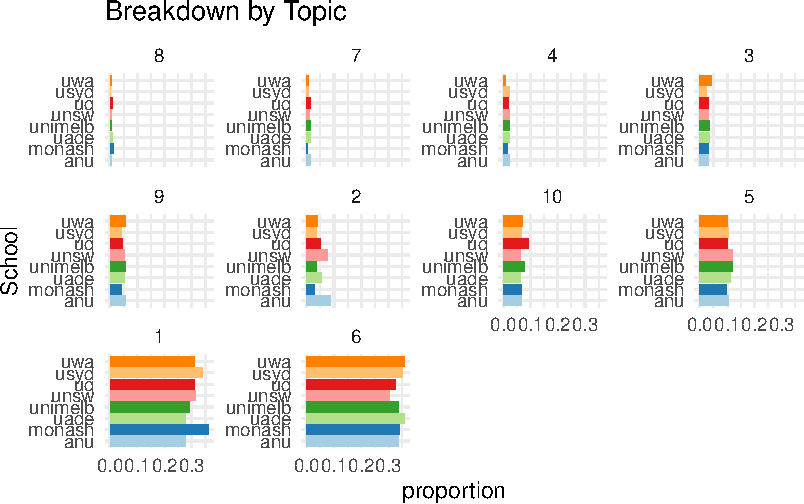
\includegraphics{./04_1-unilda_files/figure-pdf/fig-unitopics2-1.pdf}

}

\caption{\label{fig-unitopics2}Proportion Breakdown by Topic}

\end{figure}

Figure~\ref{fig-unitopics2} demonstrates a breakdown by topics instead
of universities, it is clear that compares with the results based on
only faculty in Section~\ref{sec-unit-code}, the differences between Go8
are not as much here. The proportions occupied by the eight universities
under each topic are fairly similar to each other, indicating the
subjective choice made regarding the grouping method in
Section~\ref{sec-unit-code} might have provided a slightly misleading
information, but it would require further explorations to confirm
whether it is truly the case.

\hypertarget{sec-emptopic}{%
\chapter{Apply the Selected Model to Employer Data}\label{sec-emptopic}}

To remain consistent with the analysis, we also applied the LDA model
trained by only data in statistics to the employer data with the same
stemming and standardizing procedures. Unlike the university data with
both Topic 6 and 1 as the most dominant topics, Figure~\ref{fig-emp-lda}
suggests that Topic 1 is significantly more dominant than the rest of
the topics across the different job sectors. While Topic 6 and 5
collectively takes up a large portion.

\begin{figure}

{\centering 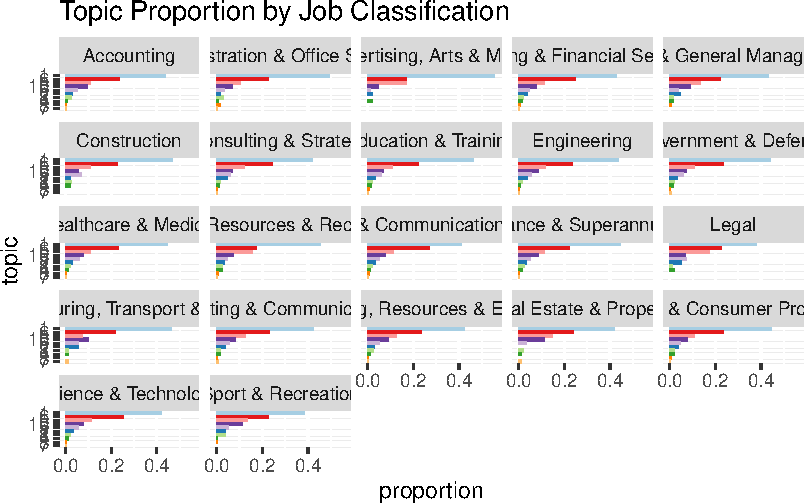
\includegraphics{./04_2-joblda_files/figure-pdf/fig-emp-lda-1.pdf}

}

\caption{\label{fig-emp-lda}Topics Proportion by Job Classification}

\end{figure}

Since the same LDA model is being applied, the breakdown of words in
each topic can be found in Figure~\ref{fig-topics}. Topic 1 has data and
statist in its top 10 words, which are also popular words found in
Figure~\ref{fig-job-freqency}. Topics 1, 6, 5 are all computational and
some statistical elements. Hence we can conclude that both the employers
universities have a more computational approach to data science.
However, the magnitude of effect for the difference in proportion of
topics is not being measured here.

\bookmarksetup{startatroot}

\hypertarget{sec-conclude}{%
\chapter{Conclusion}\label{sec-conclude}}

\hypertarget{summary}{%
\section{Summary}\label{summary}}

In this project, we collected university data and employer data to
conduct analysis. For the university data, we used web scraping
techniques to build our data set from scratch. Then, in depth
exploratory data analysis was conducted. Finally, to try and solve
problems we encountered during the analysis, we built LDA models through
web scraping over 4000 Wikipedia articles to establish our own `text
corpus'

From the exploratory data analysis, we find that Master of Data Science
degrees offered at Go8 are mostly dominated by \textbf{computational
component}, even the statistical aspects of it are more computational.
There is no obvious standard structure or skill set for data science
degrees across Go8. Hence we fail to give a definite answer on what is
universities' definition of data science in Australia. The employer's
data offered us insight to the type of programming languages are favored
by employers. We find that Python, R and SQL are the dominating ones.
Data visualization is an important skill from employers' perspective
since it appears frequently in Figure~\ref{fig-employer-bigram} and
Tableau is quite popular in Figure~\ref{fig-languages}.

Through the application of LDA model, trained with only statistical
data, we saw the breakdown of topics for employers and for universities
are slightly different. However, we lack the data and tools to measure
if the difference is significant.

\hypertarget{limitation}{%
\section{Limitation}\label{limitation}}

The research has a few limitations. The lack of data consistency within
Go8 universities lead to the small data size which made it difficult to
measure the significance the analysis. Without information on
programming languages taught at universities, we were not able to draw
direct comparison with employers.

We assumed the nature of units (computational, statistical..etc.) based
on the unit code when in reality the unit code is not a definite measure
of the content being taught. Our assumption that the content is implied
by unit code may be wrong.

A proper text corpus requires great understanding of linguistics and a
large amount of articles. The result of our LDA model topic breakdown
can also simply be due to the fact that only a few of the wiki-articles
we used are relevant and therefore will consistently be significant for
employer and university data. In addition, there are latex terms
included in the training data acquired through the web scraping process,
these terms are not fully removed and might have brought unwanted noises
to the fitted model, and possibly twisted the outputs.

We relied heavily on packages like \texttt{tidytext} and
\texttt{SnowballC} for word processing. However, there still are some
drawbacks. The stemmed words are still potentially not ``clean'' enough
and produce misleading results.

\hypertarget{furture-directions}{%
\section{Furture Directions}\label{furture-directions}}

To continue this project in the future, more degrees (e.g.~Business
Analytics) from other Australian Universities can be added to the
university data set. Also, more thought can be put into the employer
data collection. A different approach to obtaining employer data can be
considered so that the two data set is more comparable. Considering
Business analyst, data scientist, and data engineer positions. Should
these positions be put into one data set? Last but not least, more
experiments should be done with the LDA model. Such as, using different
weights for the model parameters. Other articles can also be used to
train the model. Other methodologies to convert text data into numerical
data (eg. word2vec) can also be experimented.

\bookmarksetup{startatroot}

\hypertarget{references}{%
\chapter*{References}\label{references}}
\addcontentsline{toc}{chapter}{References}

\leavevmode\vadjust pre{\hypertarget{refs}{}}%
\begin{CSLReferences}{1}{0}
Knuth (1984) R Core Team (2022) RStudio Team (2020) Landau (2021)
Selivanov, Bickel, and Wang (2022) Wickham (2022) Harrison (2022) Xie,
Cheng, and Tan (2022) Wickham et al. (2019) Silge and Robinson (2016)
Zhu (2021) Bouchet-Valat (2020) Hester and Bryan (2022) Fellows (2018)
Pedersen (2022)

\leavevmode\vadjust pre{\hypertarget{ref-snowballc}{}}%
Bouchet-Valat, Milan. 2020. \emph{SnowballC: Snowball Stemmers Based on
the c 'Libstemmer' UTF-8 Library}.
\url{https://CRAN.R-project.org/package=SnowballC}.

\leavevmode\vadjust pre{\hypertarget{ref-das2016data}{}}%
Das, Sanjiv Ranjan. 2016. {``Data Science: Theories, Models, Algorithms,
and Analytics.''} \emph{Learning} 143: 145.

\leavevmode\vadjust pre{\hypertarget{ref-wordcloud}{}}%
Fellows, Ian. 2018. \emph{Wordcloud: Word Clouds}.
\url{https://CRAN.R-project.org/package=wordcloud}.

\leavevmode\vadjust pre{\hypertarget{ref-rselenium}{}}%
Harrison, John. 2022. \emph{RSelenium: R Bindings for 'Selenium
WebDriver'}. \url{https://CRAN.R-project.org/package=RSelenium}.

\leavevmode\vadjust pre{\hypertarget{ref-glue}{}}%
Hester, Jim, and Jennifer Bryan. 2022. \emph{Glue: Interpreted String
Literals}. \url{https://CRAN.R-project.org/package=glue}.

\leavevmode\vadjust pre{\hypertarget{ref-knuth84}{}}%
Knuth, Donald E. 1984. {``Literate Programming.''} \emph{Comput. J.} 27
(2): 97--111. \url{https://doi.org/10.1093/comjnl/27.2.97}.

\leavevmode\vadjust pre{\hypertarget{ref-targets}{}}%
Landau, William Michael. 2021. {``The Targets r Package: A Dynamic
Make-Like Function-Oriented Pipeline Toolkit for Reproducibility and
High-Performance Computing.''} \emph{Journal of Open Source Software} 6
(57): 2959. \url{https://doi.org/10.21105/joss.02959}.

\leavevmode\vadjust pre{\hypertarget{ref-patchwork}{}}%
Pedersen, Thomas Lin. 2022. \emph{Patchwork: The Composer of Plots}.
\url{https://CRAN.R-project.org/package=patchwork}.

\leavevmode\vadjust pre{\hypertarget{ref-Rstats}{}}%
R Core Team. 2021. \emph{R: A Language and Environment for Statistical
Computing}. Vienna, Austria: R Foundation for Statistical Computing.
\url{https://www.R-project.org/}.

\leavevmode\vadjust pre{\hypertarget{ref-r}{}}%
---------. 2022. \emph{R: A Language and Environment for Statistical
Computing}. Vienna, Austria: R Foundation for Statistical Computing.
\url{https://www.R-project.org/}.

\leavevmode\vadjust pre{\hypertarget{ref-rstudio}{}}%
RStudio Team. 2020. \emph{RStudio: Integrated Development Environment
for r}. Boston, MA: RStudio, PBC. \url{http://www.rstudio.com/}.

\leavevmode\vadjust pre{\hypertarget{ref-text2vec}{}}%
Selivanov, Dmitriy, Manuel Bickel, and Qing Wang. 2022. \emph{Text2vec:
Modern Text Mining Framework for r}.
\url{https://CRAN.R-project.org/package=text2vec}.

\leavevmode\vadjust pre{\hypertarget{ref-tidytext}{}}%
Silge, Julia, and David Robinson. 2016. {``Tidytext: Text Mining and
Analysis Using Tidy Data Principles in r.''} \emph{JOSS} 1 (3).
\url{https://doi.org/10.21105/joss.00037}.

\leavevmode\vadjust pre{\hypertarget{ref-rvest}{}}%
Wickham, Hadley. 2022. \emph{Rvest: Easily Harvest (Scrape) Web Pages}.
\url{https://CRAN.R-project.org/package=rvest}.

\leavevmode\vadjust pre{\hypertarget{ref-tidyverse}{}}%
Wickham, Hadley, Mara Averick, Jennifer Bryan, Winston Chang, Lucy
D'Agostino McGowan, Romain Françoi, Garrett Grolemun, et al. 2019.
{``Welcome to the {tidyverse}.''} \emph{Journal of Open Source Software}
4 (43): 1686. \url{https://doi.org/10.21105/joss.01686}.

\leavevmode\vadjust pre{\hypertarget{ref-dt}{}}%
Xie, Yihui, Joe Cheng, and Xianying Tan. 2022. \emph{DT: A Wrapper of
the JavaScript Library 'DataTables'}.
\url{https://CRAN.R-project.org/package=DT}.

\leavevmode\vadjust pre{\hypertarget{ref-kableextra}{}}%
Zhu, Hao. 2021. \emph{kableExtra: Construct Complex Table with 'Kable'
and Pipe Syntax}. \url{https://CRAN.R-project.org/package=kableExtra}.

\end{CSLReferences}



\end{document}
